%%%%%%%%%%%%%%%%%%%%%%%%%%%%%%%%%%%%%%%%%%%%%%%%%%%%%%%%%%%%%
%%%%%% Article draft for submission to ISeCure Journal %%%%%%
%%%%%%%%%%%%%%%%%%%%%%%%%%%%%%%%%%%%%%%%%%%%%%%%%%%%%%%%%%%%%
\documentclass[Print]{../Style/isecure-v24}

\pdfminorversion=4
%\usepackage{amsmath,amssymb}
%\usepackage{array}
\usepackage{lipsum}
\usepackage{algpseudocode,algorithm}
\usepackage[colorlinks, bookmarksnumbered, linkcolor=darkblue, citecolor=darkred, urlcolor=darkgreen]{hyperref}
\usepackage[numbers,sort&compress]{natbib}
\usepackage[all]{hypcap}
\usepackage{../Style/picins}
\usepackage{lettrine}
\usepackage{wrapfig}
\usepackage{graphicx}
\usepackage{subcaption}
%\usepackage{multicol}

%\hypersetup{colorlinks=true}
\usepackage{amsthm}
\usepackage{amssymb,amsmath,amsfonts,eqnarray,breqn}
\usepackage{fancyhdr}
%\usepackage{cite}
\usepackage{ragged2e}
\usepackage{enumitem}   
\usepackage{refcount}
\usepackage[protrusion=true,expansion=true]{microtype}
\usepackage{float}
\usepackage[greek,english]{babel}
\usepackage[LGR,T1]{fontenc}
%%%%%%%%%%%%%%%%%%%%%%%%%%%%%%%%%%%%%%%%%%%%%%%%%%%%%%%%%%%%%%%%%%%%%%%%%
%\theoremstyle{plain}

\DisableLigatures[f]{encoding=*,family=*}
\graphicspath{{Images/},{../Style/}}
\DeclareGraphicsExtensions{.jpg,.pdf,.png}
\RequirePackage{amsthm}%
\def\th@plain{%
\thm@preskip\parskip
\thm@postskip\z@
\itshape % body font
}
\def\th@definition{%
\thm@preskip\parskip
\thm@postskip\z@
\normalfont % body font
}
\def\th@remark{%
\thm@headfont{\itshape}%
\normalfont % body font
\thm@preskip\parskip \divide\thm@preskip\tw@
\thm@postskip\z@
}

%\newenvironment{pf}%
%  {\par\addvspace{\@bls \@plus 0.5\@bls \@minus 0.1\@bls}\noindent
%   {\bfseries\Elproofname}\enspace\ignorespaces}%
%  {\par\addvspace{\@bls \@plus 0.5\@bls \@minus 0.1\@bls}}
%\def\Elproofname{PROOF.}
%\@namedef{pf*}#1{\par\begingroup\def\Elproofname{#1}\pf\endgroup\ignorespaces}
%\expandafter\let\csname endpf*\endcsname=\endpf


\newtheoremstyle{XYZ}% name
{3pt}% Space above
{3pt}% Space below
{}% Body font
{}% Indent amount
{\bfseries}% Theorem head font
{}% Punctuation after theorem head
{.5em}% Space after theorem head
{\bfseries{#1 #2\if#3\else~(#3)\fi.}}% Theorem head spec (can be left empty, meaning `normal')



\theoremstyle{plain}
\newtheorem{theorem}{Theorem}
\newtheorem{proposition}{Proposition}
\newtheorem{corollary}{Corollary}
\newtheorem{lemma}{Lemma}
\newtheorem{claim}{Claim}
\newtheorem{axiom}{Axiom}
\newtheorem{conjecture}{Conjecture}
\newtheorem{fact}{Fact}
\newtheorem{hypothesis}{Hypothesis}
\newtheorem{assumtion}{Assumption}
\newtheorem{criterion}{Criterion}
\theoremstyle{XYZ}
\newtheorem{definition}{Definition}
\newtheorem{example}{Example}
\newtheorem{remark}{Remark}
\newtheorem{notation}{Notation}
\newtheorem{problem}{Problem}
\newtheorem{principle}{Principle} 
\articletype{Short Paper}
\def\sectionautorefname{Section} % localizing \autoref{}
\def\subsectionautorefname{Section} % localizing \autoref{}
\def\subsubsectionautorefname{Section} % localizing \autoref{}
\providecommand*{\lemmaautorefname}{Lemma}
%\newcommand{\subsubsectionautorefname}{Section}
\usepackage{titlesec}
\setcounter{secnumdepth}{4}
\titleformat{\paragraph}
{\normalfont\normalsize\bfseries}{\theparagraph}{1em}{}
\titlespacing*{\paragraph}
{0pt}{3.25ex plus 1ex minus .2ex}{1.5ex plus .2ex}

\journal{ISeCure}
\company{ISC}
\copyrightyear{2018}
\journalsite{\href{https://github.com/RavinduMPK/Deep-Learning-Based-Detection-and-Localization-of-Intracranial-Hemorrhage-Types}{\footnotesize GitHub Repository}}
\firstpage{1} % TODO



\makeatletter
\begingroup \lccode`+=32 \lowercase
 {\endgroup \def\Url@ObeySp{\Url@Edit\Url@String{ }{+}}}
 \def\Url@space{\penalty\Url@sppen\ }
\makeatother


%%%%% Use the following commands for putting a watermark
%\usepackage{type1cm}
%\usepackage{eso-pic}
%\makeatletter
%\AddToShipoutPicture{
%            \setlength{\@tempdimb}{.5\paperwidth}
%            \setlength{\@tempdimc}{.5\paperheight}
%            \setlength{\unitlength}{1pt}
%            \put(\strip@pt\@tempdimb,\strip@pt\@tempdimc){
%        \makebox(600,-900){\rotatebox{45}{\textcolor[gray]{0.90}
%        {\fontsize{2cm}{2cm}\selectfont{\bfseries{Uncorrected~~~~Proof}}}}}
%            }
%}
%\makeatother

%Use the following command for putting line numbers
\usepackage[displaymath]{lineno}  %DON'T COMMENT EVEN IF YOU DONT WANT LINE NOS
\newcommand*\patchAmsMathEnvironmentForLineno[1]{
  \expandafter\let\csname old#1\expandafter\endcsname\csname #1\endcsname
  \expandafter\let\csname oldend#1\expandafter\endcsname\csname end#1\endcsname
   \renewenvironment{#1}
     {\linenomath\csname old#1\endcsname}
     {\csname oldend#1\endcsname\endlinenomath}}
\newcommand*\patchBothAmsMathEnvironmentsForLineno[1]{
  \patchAmsMathEnvironmentForLineno{#1}
  \patchAmsMathEnvironmentForLineno{#1*}}
\AtBeginDocument{
\patchBothAmsMathEnvironmentsForLineno{equation}
\patchBothAmsMathEnvironmentsForLineno{align}
\patchBothAmsMathEnvironmentsForLineno{flalign}
\patchBothAmsMathEnvironmentsForLineno{alignat}
\patchBothAmsMathEnvironmentsForLineno{gather}
\patchBothAmsMathEnvironmentsForLineno{multline}
}

%%%%%%%%%%%%%%%%%%%%%%%%%%%%%%%%%%%%%%%%%%%%%%%%%%%%%%%%%%%%%%%%%%%%%%%%

%%%%%%%%%%%%%%%%%%%%%%%%%%%%%%%%%%%%%%%%%%%%%%%%%%%%%%%%%%%%%%%%%%%%%
\newtheorem{cor}{Corollary}[section]
\newtheorem{exmp}{Example}[section]
\newtheorem{construction}{Construction}[section]
\newtheorem{defn}{Definition}[section]
\newcommand*\concat{\mathbin{\|}}
%%%%%%%%%%%%%%%%%%%%%%%%%%%%%%%%%%%%%%%%%%%

\begin{document}
%\linenumbers
\begin{frontmatter}

%------------------- Paper Title ------------------------------
% Titles are generally capitalized except for words such as a, an, and, as, at, but, by, for, in, nor, of, on, or, the, to and up, which are usually not capitalized unless they are the first or last word of the title. Linebreaks \\ can be used within to get better formatting as desired. Do not put math or special symbols in the title. Title of up to 17 words should not contain the name of locations, countries or cities of the research as well as abbreviations. Avoid complicated and technical expressions and do not use vague expressions. The title should be oriented to ISeCure scope issues while not being obscure or meaningless.

\def\NoDingTitle{Deep Learning-Based Detection and Localization of Intracranial Hemorrhage Types}
\title{\NoDingTitle\textsuperscript{ }}

%------------------- Author names and Affiliations ------------------------------
% Add your name, affiliations and email in this part. Please consider that an academic email is preferred. If the fisrt author isn't corresponding author in your case, please set the CorAuth option in \author command for that author. 

\author[a1,CorAuth]{Pushpakumara H.M.R.M.}, and%
\ead{ pushpakumarahmrm.20@uom.lk}
\author[a2]{Tilakarathna U.A.}
\ead{ tilakarathnaua.20@uom.lk}


\address[a1]{Dep. of Electronic and Telecom. Engineering, University of Moratuwa, Sri Lanka.}
\address[a2]{Dep. of Electronic and Telecom. Engineering, University of Moratuwa, Sri Lanka.}

\corauth[CorAuth]{Corresponding author.}% Do not change this field.



%------------------- Abstract ------------------------------
\begin{abstract}
This study explores an application of deep learning, for the detection and classification of intracranial hemorrhages in non-contrast head CT scans. Utilizing the Brain Hemorrhage Extended (BHX) dataset, the images undergo preprocessing, and the YOLOv8 model demonstrates its efficacy in accurately predicting and localizing hemorrhages, even in scenarios with multiple labels per image. The study discusses key parameters, model architecture, and potential future works, contributing to advancements in AI for medical imaging and timely clinical interventions.

%% The following command generate a random text.
\end{abstract}

%---------------------- Keywords -------------------------------
% Please provide 3 to 5 keywords, each separated by hyphen and started in capital letter.
\begin{keyword}
YOLO \\
Intracranial hemorrhage\\
CT\\
Deep learning\\
Bounding box

\end{keyword}


\makeatother

\end{frontmatter}

\addtolength{\parskip}{2mm}

%---------------------- Introduction ---------------------------

\section{Introduction} \label{sec:intro}

Intracranial hemorrhage (ICH) stands as a significant medical event, constituting up to 15\% of strokes. With an incidence rate of around 25 per 100,000 person-years and a mortality rate of 40\% within one month of presentation, ICH demands careful attention. It can manifest in various intracranial compartments due to diverse pathology. Neuroimaging becomes crucial for physicians, aiding in understanding the hemorrhage's location, volume, the risk of impending cerebral injury, and guiding emergent patient treatment. Non-contrast head CT scans are among the most commonly used emergency room diagnostic tools for patients with head injury or for those with symptoms suggesting a stroke or rise in intracranial pressure. The wide availability and low acquisition time of these scans make them a commonly used first-line diagnostic method. 

Deep learning has showcased remarkable accuracy in classifying and detecting medical conditions from raw images. Its successful application extends to brain diseases like tumors and hemorrhages. The bounding box generated by deep learning not only pinpoints the location, height, and width of the hemorrhage but also furnishes valuable information for diagnosis, aiding experts in anomaly detection within the brain. \\
Here, we use the Brain Hemorrhage Extended (BHX): Bounding box extrapolation from thick to thin slice CT images dataset, which contains the annotated bounding boxes of 6 hemorrhage types. Here, we pre-process the images by converting them to usable formats, removing noise and further processing as mentioned below, and then we feed the images to the YOLOv8 object detection algorithm, which is our deep learning model to identify the hemorrhages. 




\section{Material and Method} \label{sec:material and method}
\subsection{Dataset} \label{sec:Dataset} 
Our dataset used, BHX, contains up to 39,668 bounding boxes in 23,409 images annotated for hemorrhage, out of a total of 170k images from the qure.ai CQ500 dataset. There are labels for each of the 5 different types of acute hemorrhage: Intraparenchymal, Subarachnoid, Intraventricular, Epidural, and Subdural, and an extra sixth label for Chronic Subdural Hematoma. Examples of intracranial hemorrhages and boxes are shown in Figure \ref{fig:labels}.
There are three versions of labels. We have used the clean version. It has mitigated inconsistencies between different CT acquisitions, related to minor movements during the examination. It also does not contain the bone filtered images, which are suboptimal for hemorrhage assessment. The clean dataset contains 27,203 bounding box on 15,979 images. In this set of bounding boxes, there are multiple labels for a single image. Likewise, in our predictions we have predictions in a similar manner, with multiple predictions shown in a single image. 

\subsection{ Methodology} \label{sec: Methodology} 
The methodology employed in this study involved the utilization of deep learning techniques to detect and localize hemorrhage types within head CT scan images. The CQ500 Head CT images dataset served as the source of annotated CT scan images, which underwent preprocessing to mitigate noise and enhance image quality. Subsequently, a pre-trained deep learning network was employed for training purposes. The training data comprised 80\% of the preprocessed images, while the remaining 20\% constituted the testing data. The trained deep learning model was then tasked with generating bounding boxes, indicating the location and extent of hemorrhage regions within the CT scan images. 
The employed method is summarized in Figure \ref{fig:employed_method}. Each of the steps given in Figure \ref{fig:employed_method} was described in the next sections.

\subsection{Preprocessing} \label{sec: Preprocessing}
\subsubsection{Pixel Value Transformation to Hounsfield Unit (HU)}
The first step in the preprocessing pipeline is to transform the pixel values in the CT scan image from their original format to Hounsfield Units (HU). Converting the pixel values to HU ensures that the images are represented in a consistent and standardized manner, which is crucial for subsequent processing and analysis.
\subsubsection{Windowing}
Since the HU range for CT scans can be quite large (typically around -1000 to 4000 HU), it is often impractical to display the entire range of values in a single image. We used windowing technique to adjust the range of pixel values that are displayed in an image, effectively zooming in on a specific range of interest.
We used a window level of 40 and a window width of 80. This means that only HU values between -20 and 60 will be displayed, while values outside this range will be clipped to the minimum and maximum values, respectively. This  compresses the HU range and enhances brain tissue contrast.
\subsubsection{Normalization}
After applying windowing, the pixel values in the image are normalized to the range of [0, 255]. This is important to ensure that the pixel values can be represented as 8-bit integers.
\subsubsection{Morphology Dilation}
We applied morphology dilation to the image by using a 3x3 kernel. This kernel is small enough to preserve the overall shape of the brain tissue, while also effectively removing small noise particles.
\subsubsection{Dimension Squeezing}
After dilation, the image might have an extra dimension, which can be unnecessary for further analysis. Here we squeezed the image arrays from 3D to 2D.\\

\subsection{Data Preparations for training} \label{sec: Data prep}
In the CQ500 dataset, it was observed that certain medical images contained multiple instances of brain hemorrhages, each corresponding to a different type or category. To address this, a data preprocessing strategy was employed, involving the separation of individual annotations for each type of hemorrhage present in such images.
Consequently, for images with multiple annotations, the same image was introduced into the training pipeline multiple times, with each iteration dedicated to a different annotation. This practice ensured that the deep learning model could discern and annotate each type of hemorrhage independently, even within the same image context.
This approach was implemented to enhance the model's capacity to accurately detect and classify various types of brain hemorrhages, considering the unique characteristics of each, even when co-occurring within a single image. Despite the necessity of repetitive presentation of identical images with distinct annotations, the method contributed to improving the model's ability to handle multifaceted scenarios in medical image analysis, ultimately enhancing its diagnostic capabilities.

As shown in Figure \ref{fig:label-count}, when we observe this, we can see the class imbalance is not a big issue except for the Epidural class.  

At the end, we had 21751 (80\%) images for training and 5438 (20\%) images for validation.

And also, since we used YOLOv8 as our model, we had to resize our images from 512x512 to 640x640 pixels to meet the model's requirements.

\newpage
\onecolumn
{\begin{figure}[h]
    \centering
    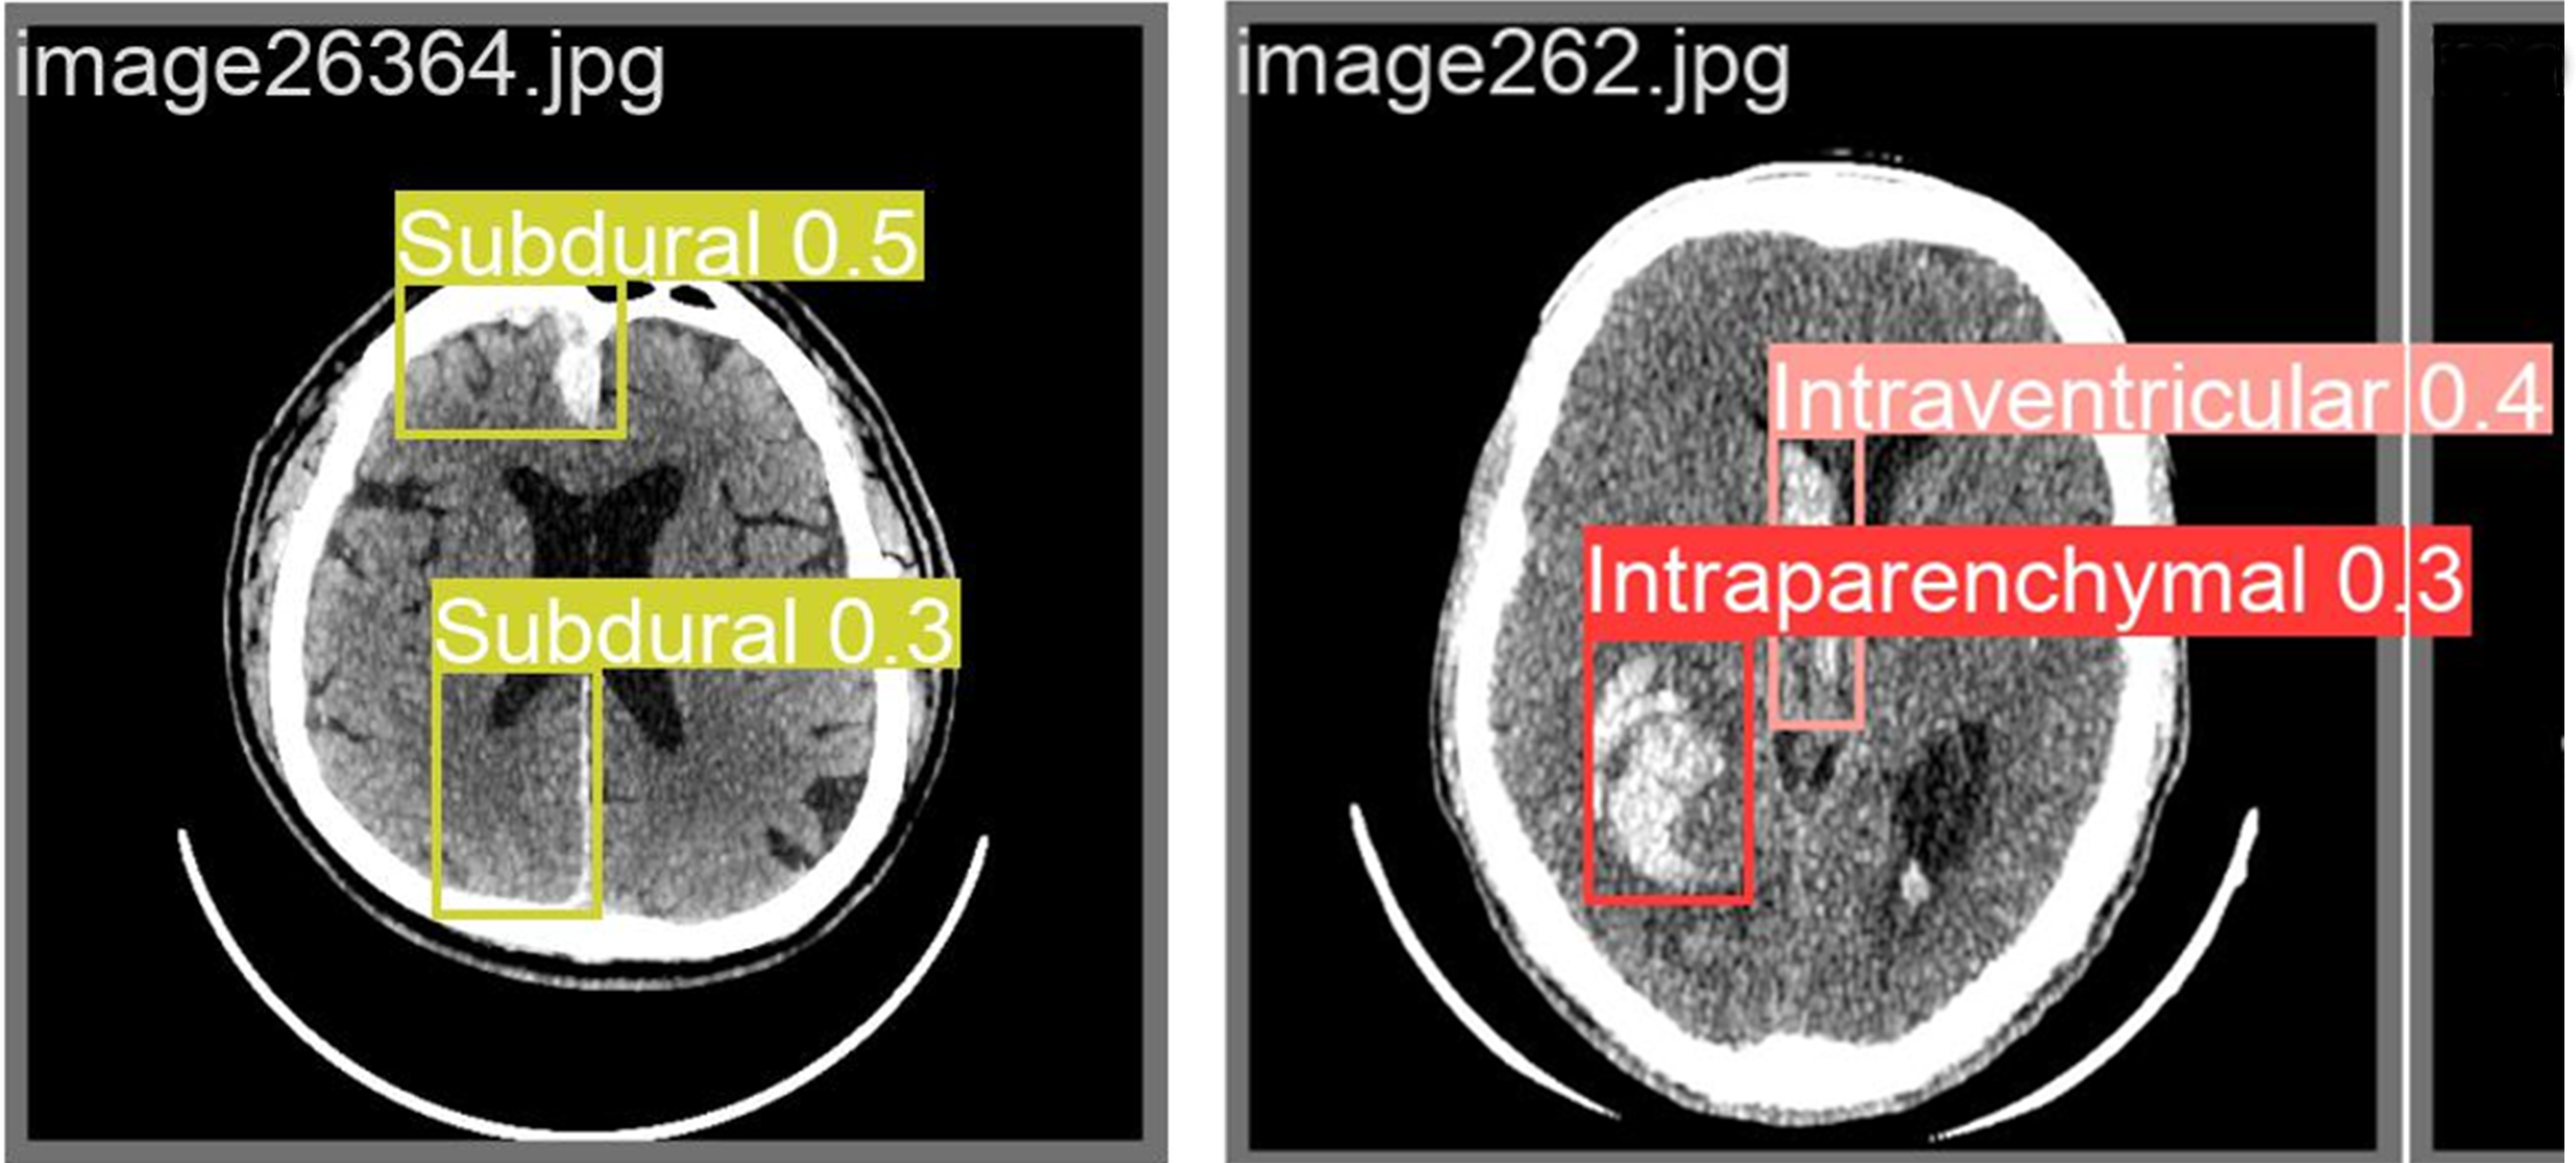
\includegraphics[width=1.0\linewidth]{ISeCure Draft/Images/edited.png}
    \captionsetup{font=small}
    \caption{Examples of intracranial hemorrhages and boxes: image26354) two boxes with single types of hemorrhage in one image (Subdural),
image262) two boxes with two different types of hemorrhage in one image (Intraventricular, Intraparenchymal).}
    \label{fig:labels}
\end{figure}}

{\begin{figure}[h]
    \centering
    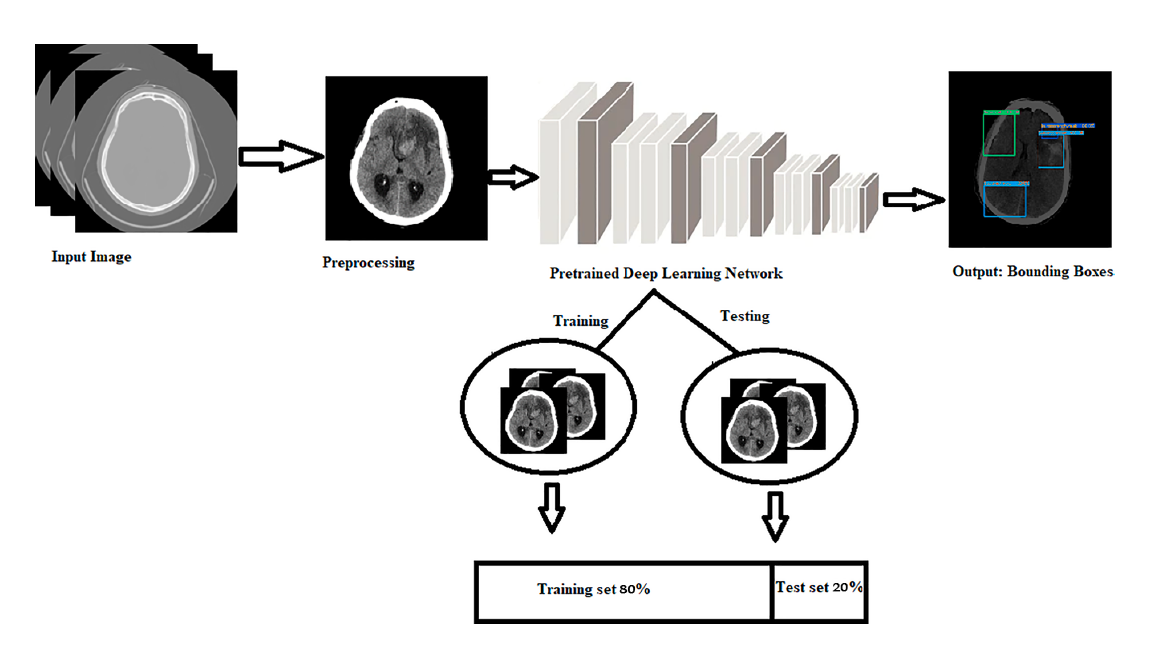
\includegraphics[width=1.0\linewidth]{ISeCure Draft/Images/model.png}
    \captionsetup{font=small}
    \caption{Employed methodology diagram.}
    \label{fig:employed_method}
\end{figure}}
\newpage
{\begin{figure}[h]
    \centering
    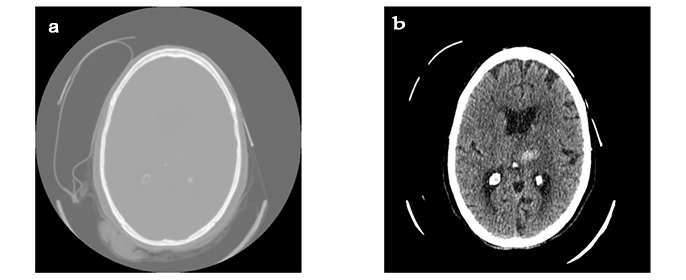
\includegraphics[width=1.0\linewidth]{ISeCure Draft/Images/NAP.png}
    \captionsetup{font=small}
    \caption{a) Normal Image. b) Pre-processed Image.}
    \label{fig:normal and processed}
\end{figure}}

{\begin{figure}[h]
    \centering
    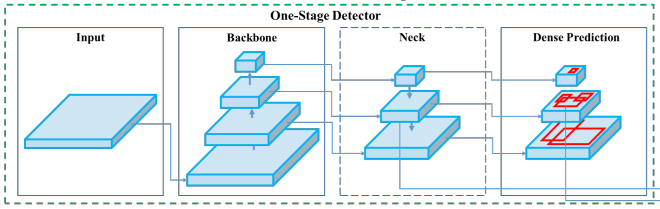
\includegraphics[width=1.0\linewidth]{ISeCure Draft/Images/OSD.png}
    \captionsetup{font=small}
    \caption{Typical one-stage object detector architecture.}
    \label{fig:one stage od}
\end{figure}}

{\begin{figure}[h]
    \centering
    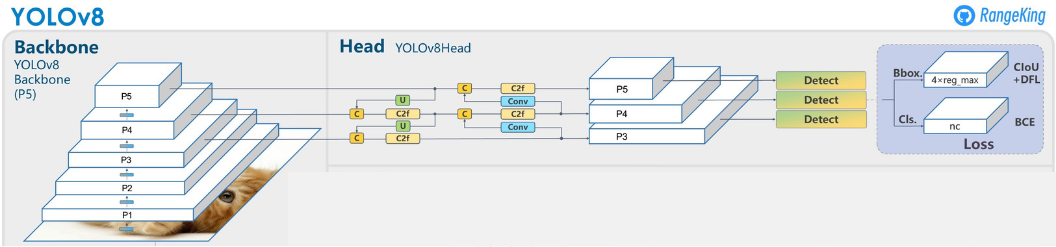
\includegraphics[width=1.0\linewidth]{ISeCure Draft/Images/yolov8.png}
    \captionsetup{font=small}
    \caption{YOLOv8 architecture.}
    \label{fig:yolov8}
\end{figure}}

\newpage
{\begin{figure}[h]
    \centering
    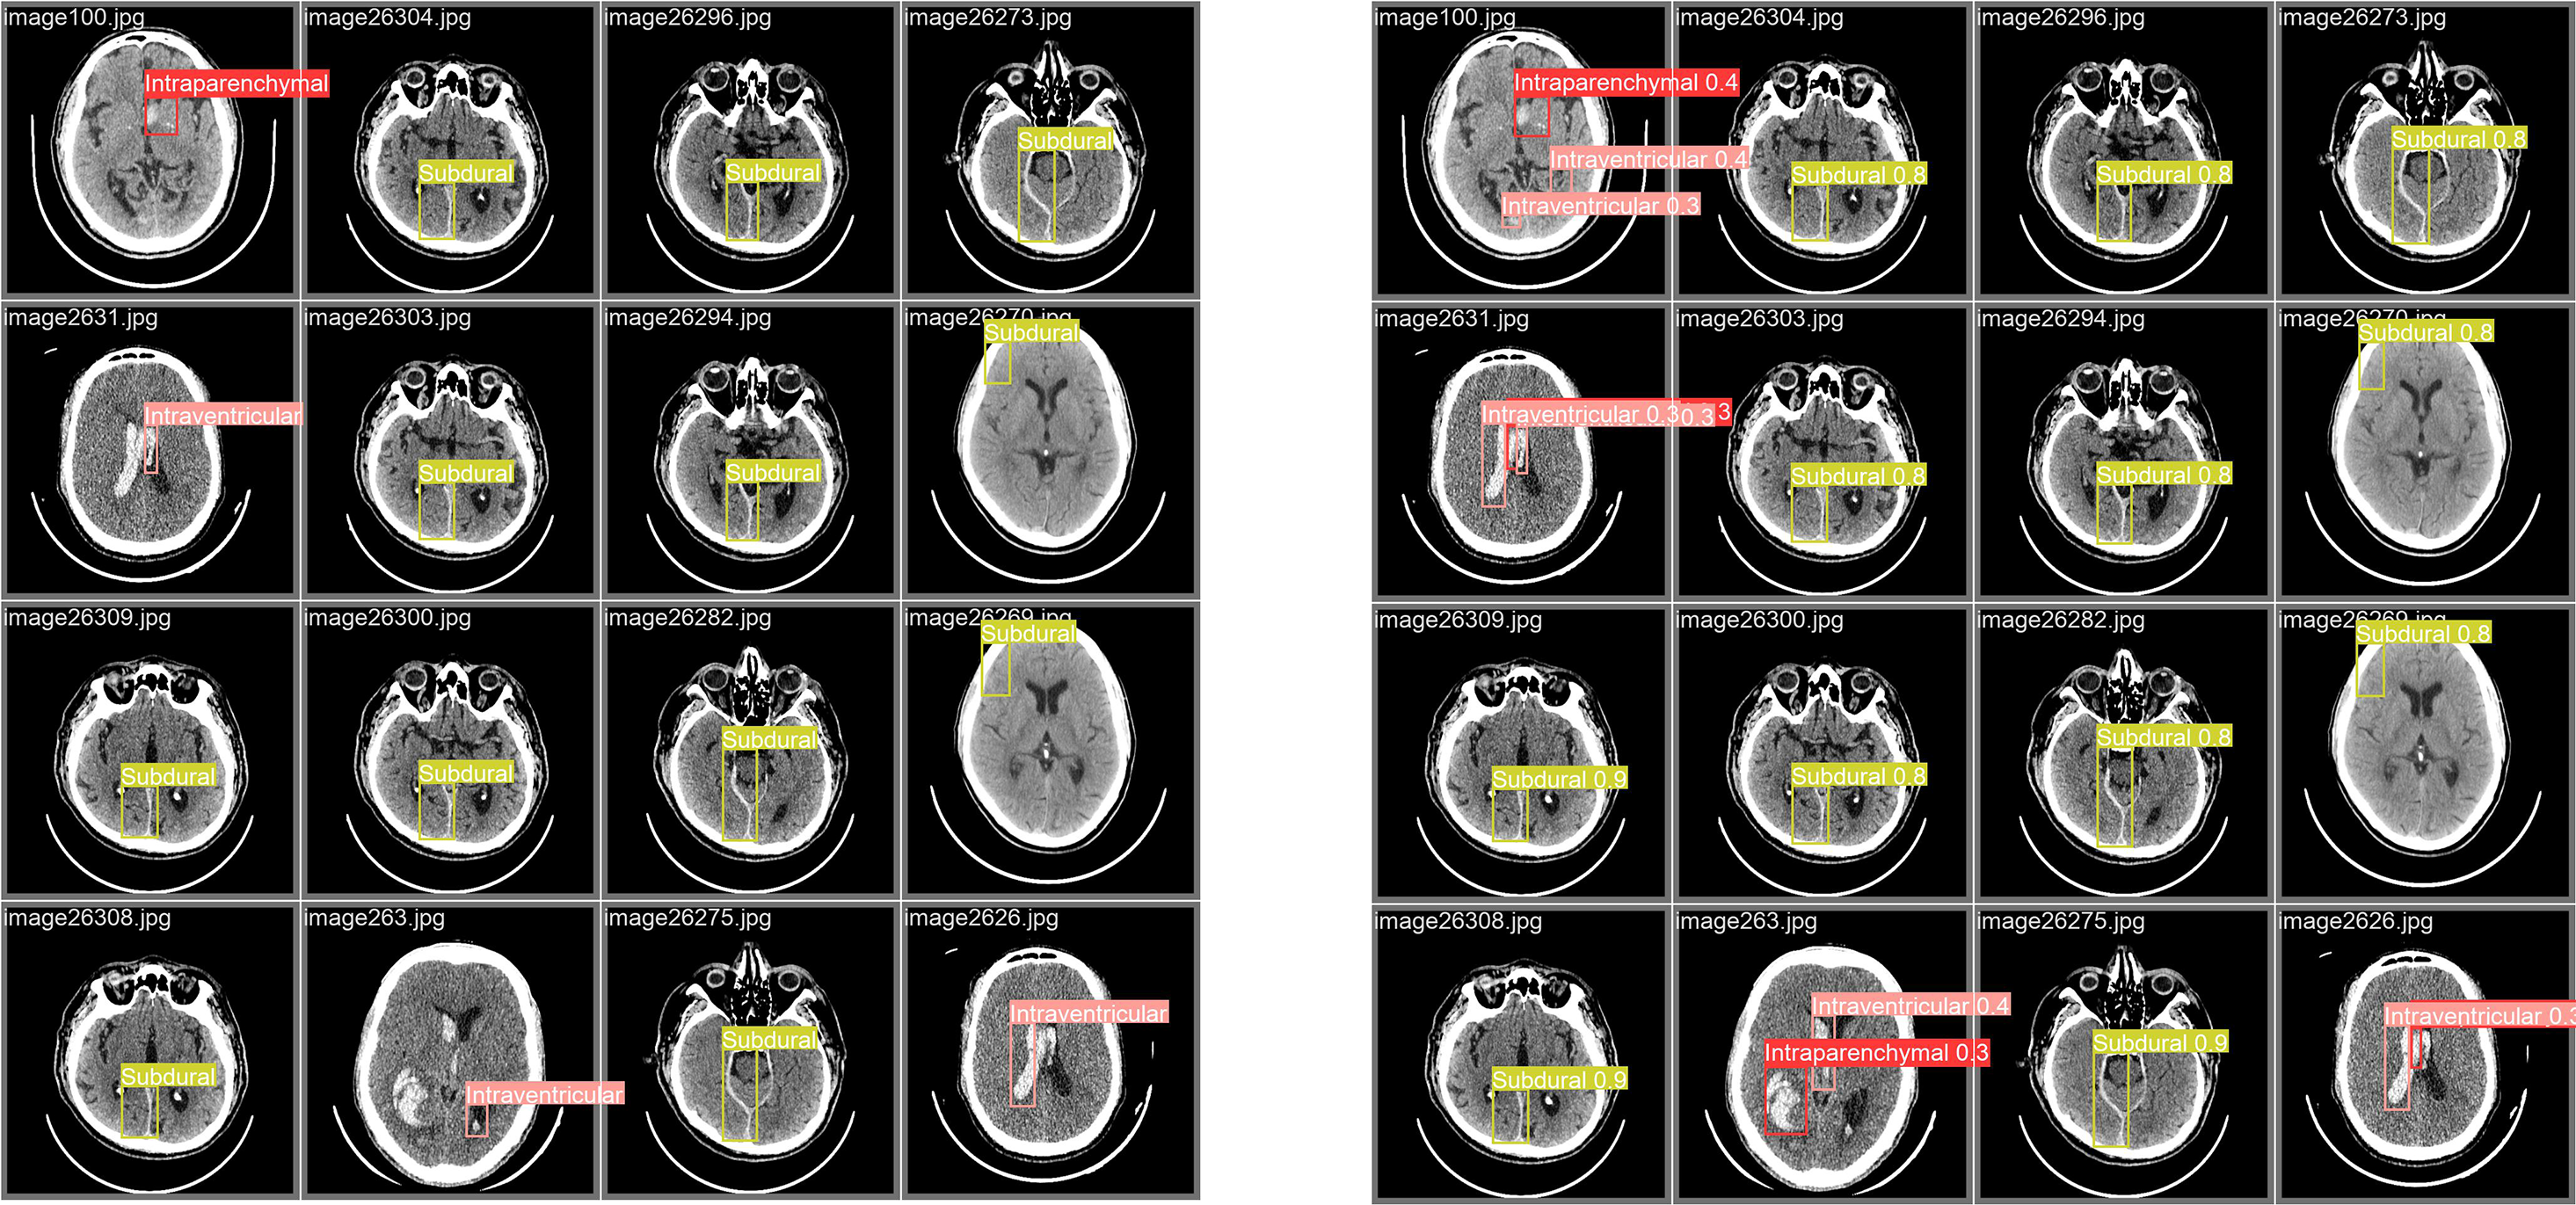
\includegraphics[width=1.0\linewidth]{ISeCure Draft/Images/OrvPrd.png}
    \captionsetup{font=small}
    \caption{LHS: Original Labels. RHS: Predicted Labels}
    \label{fig:OvP}
\end{figure}}

{\begin{figure}[h]
    \centering
    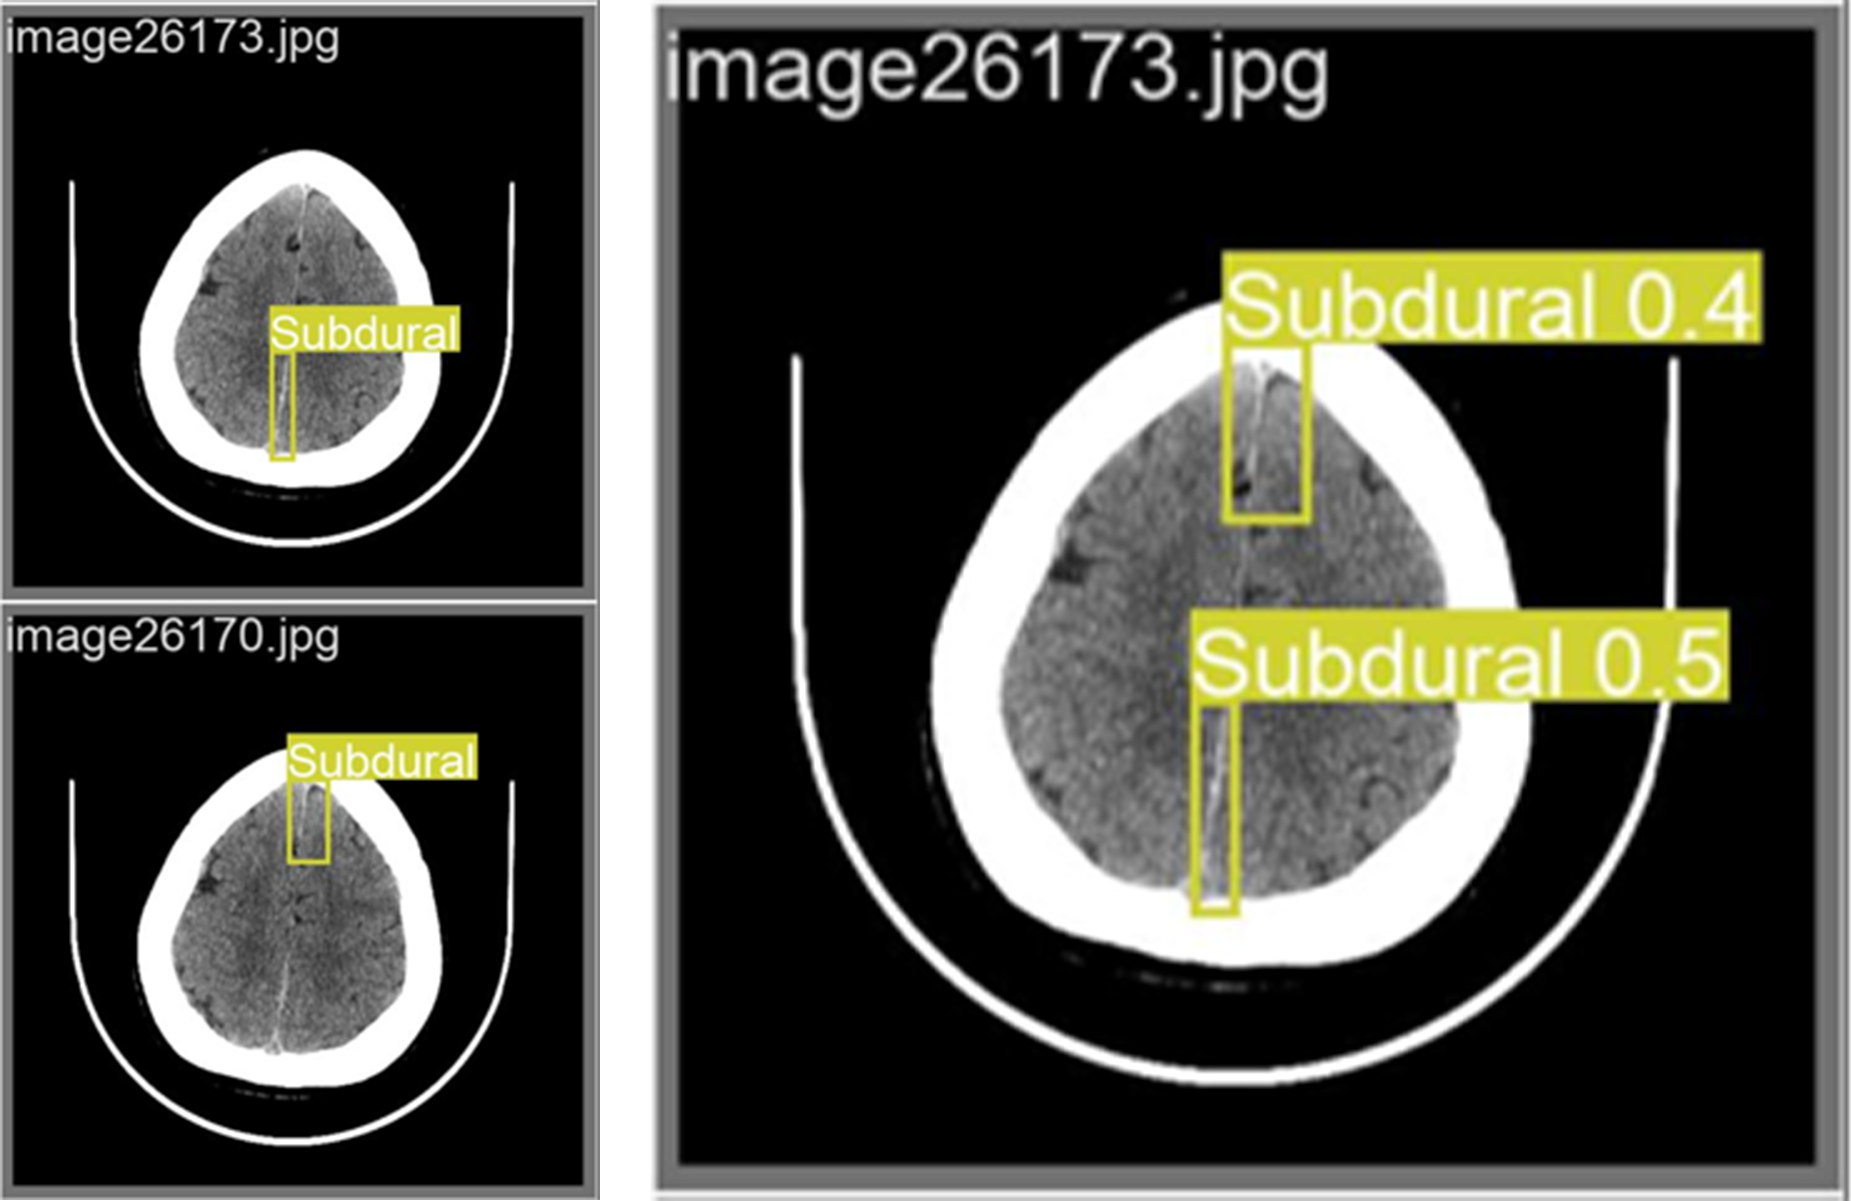
\includegraphics[width=1.0\linewidth]{ISeCure Draft/Images/two_sep.png}
    \captionsetup{font=small}
    \caption{Two separated labels in data (LHS) and Correctly Predicted two separate hemorrhages (RHS)}
    \label{fig:two_sep}
\end{figure}}

\newpage
\twocolumn

{\begin{figure}[h]
    \centering
    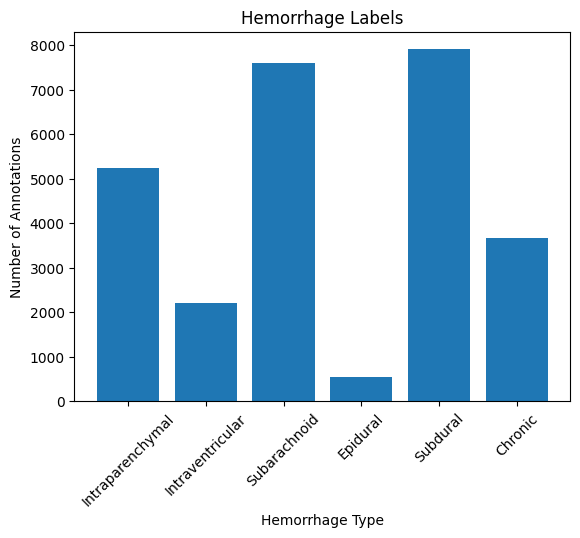
\includegraphics[width=1.0\linewidth]{ISeCure Draft/Images/output.png}
    \captionsetup{font=small}
    \caption{Number of labels.}
    \label{fig:label-count}
\end{figure}}

\subsection{YOLOv8} \label{sec:yolo}
YOLOv8, or "You Only Look Once version 8," represents a significant advancement in the realm of object detection algorithms.  Here, we use the ultralytics YOLOv8. Ultralytics YOLOv8 is the latest version of the YOLO object detection and image segmentation model developed by Ultralytics. YOLOv8 is also highly efficient and can be run on a variety of hardware platforms, from CPUs to GPUs. The architecture of YOLOv8 builds upon the previous versions of YOLO algorithms. YOLOv8 utilizes a convolutional neural network that can be divided into two main parts: the backbone and the head. 
A modified version of the CSPDarknet53 architecture forms the backbone of YOLOv8. This architecture consists of 53 convolutional layers and employs cross-stage partial connections to improve information flow between the different layers. The head of YOLOv8 consists of multiple convolutional layers followed by a series of fully connected layers. These layers are responsible for predicting bounding boxes, objectness scores, and class probabilities for the objects detected in an image.
One of the key features of YOLOv8 is the use of a self-attention mechanism in the head of the network. This mechanism allows the model to focus on different parts of the image and adjust the importance of different features based on their relevance to the task.
Another important feature of YOLOv8 is its ability to perform multi-scaled object detection. The model utilizes a feature pyramid network to detect objects of different sizes and scales within an image. This feature pyramid network consists of multiple layers that detect objects at different scales, allowing the model to detect large and small objects within an image.

Another notable aspect of YOLOv8 is its ensemble approach. By combining predictions from models of different sizes and complexities, the algorithm enhances its ability to generalize and detect objects under diverse conditions. This ensemble strategy is particularly advantageous in scenarios where objects may exhibit varying characteristics, lighting conditions, or orientations.

In the training phase, YOLOv8 incorporates advanced techniques tailored for optimal object detection performance. Mosaic data augmentation is one such method, where multiple images are fused into one, enriching the model's ability to recognize diverse object configurations. Additionally, the use of CIoU loss (Complete Intersection over Union) during training contributes to improved bounding box regression, leading to more accurate localization of objects.

We used the YOLOv8 model to train our preprocessed images mentioned before, and detect the hemorrhages. For this, we feed the images, and also the labeled files required to train the model.


\section{Results and Discussions} \label{sec:results and discussion}
\subsection{Employed parameters} \label{sec: Employed parm}
The proposed hemorrhage detection model was trained using the CQ500 dataset, which comprises annotated CT scan images. The model was trained incrementally, gradually increasing the number of epochs to account for the dataset's substantial size. During training, pre-trained weights were employed to initialize the detection network, followed by fine-tuning the network to adapt it to the specific task of hemorrhage detection. The training process was terminated when the loss function converged, as depicted in Figure 9. The training employed stochastic gradient descent (SGD) optimization with the Adam optimizer, utilizing an initial learning rate of 0.01 and batch sizes of 16. Figure \ref{fig:loss}

{\begin{figure}[h]
    \centering
    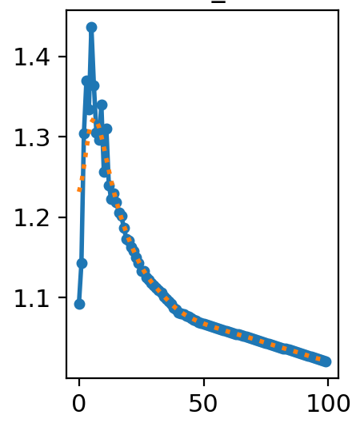
\includegraphics[width=1.0\linewidth]{ISeCure Draft/Images/lve250_350.png}
    \captionsetup{font=small}
    \caption{Loss from 250 - 350 (epochs)}
    \label{fig:loss}
\end{figure}}

The proposed model architecture comprises 225 layers, resulting in a total of 3,012,018 learnable parameters and 3,012,002 gradients.

All detection models were trained and evaluated on a cloud-based computing environment utilizing Kaggle GPU T4 x2 instances with 16GB RAM.

\subsection{Detecting bounding boxes and hemorrhage types} \label{sec:bounding box detect}

In this project, we used the YOLOv8 algorithm to perform a detection task for different types of brain hemorrhage. Figure \ref{OvP} show some examples of predicted and ground truth boxes.
Even though we used a single label per image for the training process, the model was able to correctly predict multiple labels in a single scan, as clearly demonstrated in Figure \ref{fig:OvP}. Also, we can see multiple bounding boxes are also have correctly predicted in there. Figure \ref{fig:two_sep}
This result is significant because it shows that YOLOv8 can be used to detect multiple hemorrhages in a single scan, even when the training dataset only contains images with a single label. This is important for clinical applications, where it is crucial to identify all hemorrhages present in an image. For better understanding, refer the confusion matrix. Figure \ref{fig:cm}

{\begin{figure}[h]
    \centering
    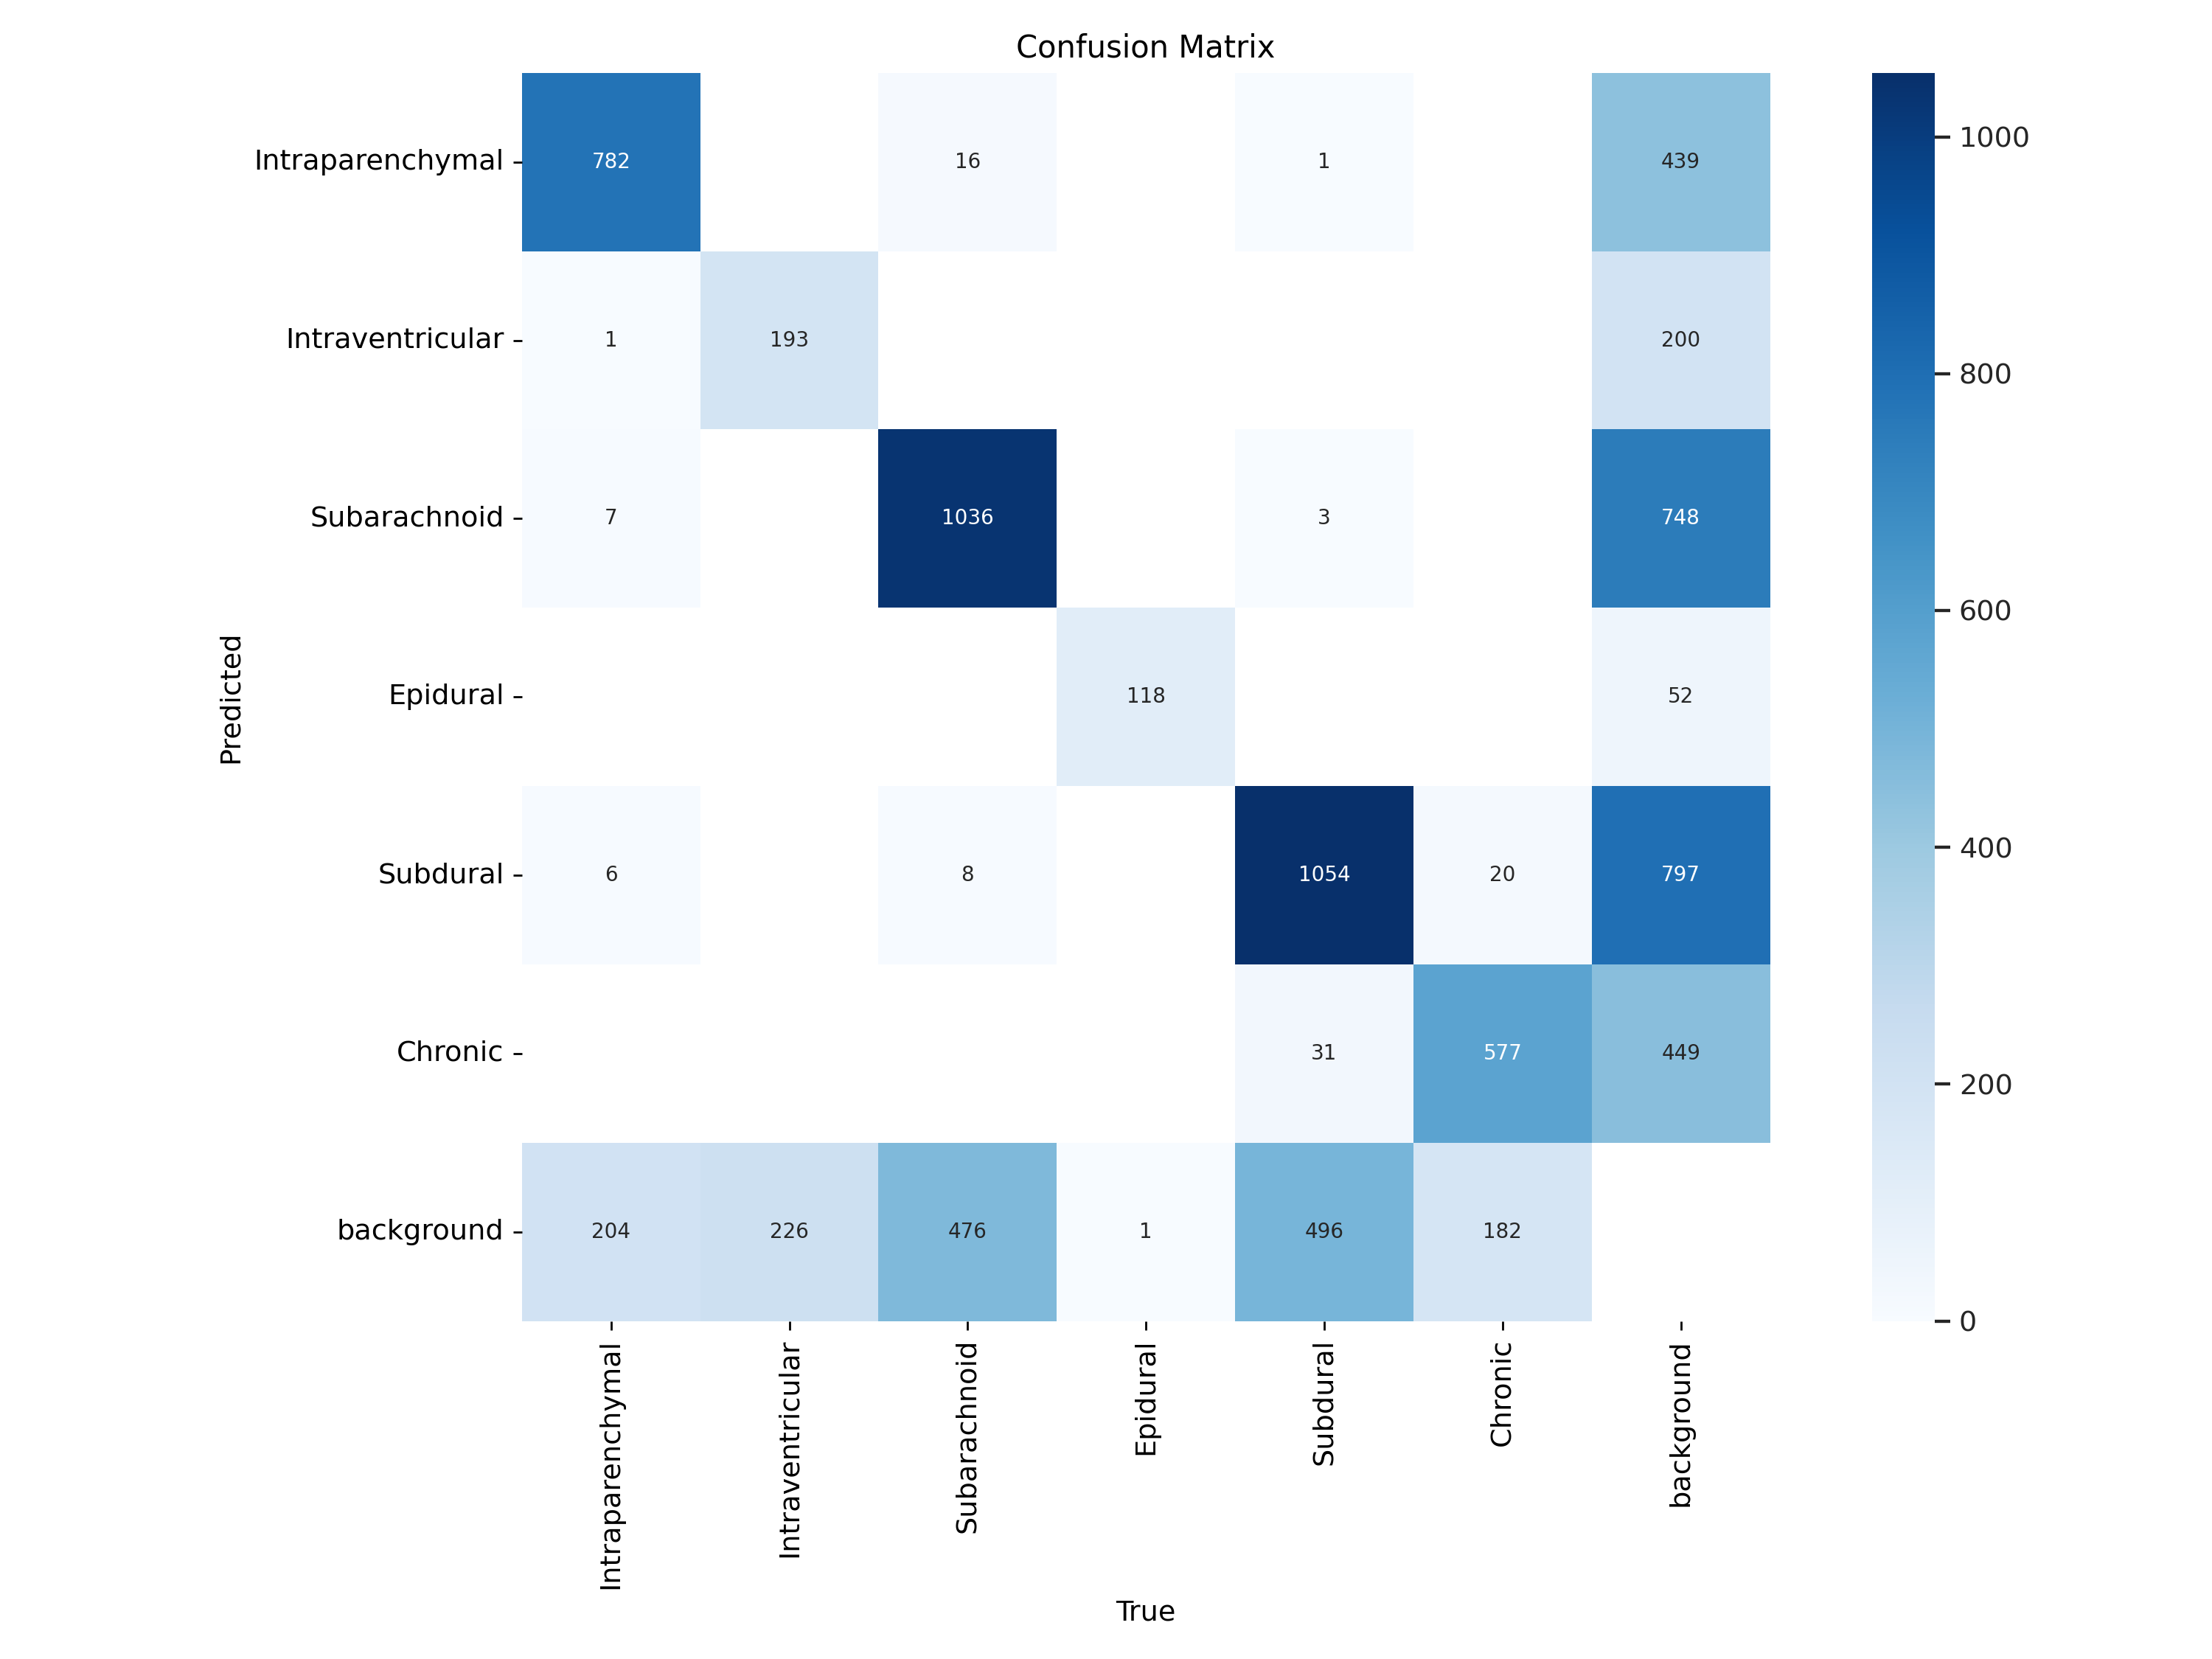
\includegraphics[width=1.0\linewidth]{ISeCure Draft/Images/cm.png}
    \captionsetup{font=small}
    \caption{confusion matrix}
    \label{fig:cm}
\end{figure}}

\subsection{Comparison} \label{sec: comparison}
We observed that the precision of the  model increased as we increased the number of epochs trained. However, we were limited by the GPU resources available to us, and were unable to train the model for as many epochs as we would have liked. Therefore, we believe that it is possible to achieve even higher precision by training the model for more epochs.

The following plots summarize the results we obtained for the model.

{\begin{figure}[h]
    \centering
    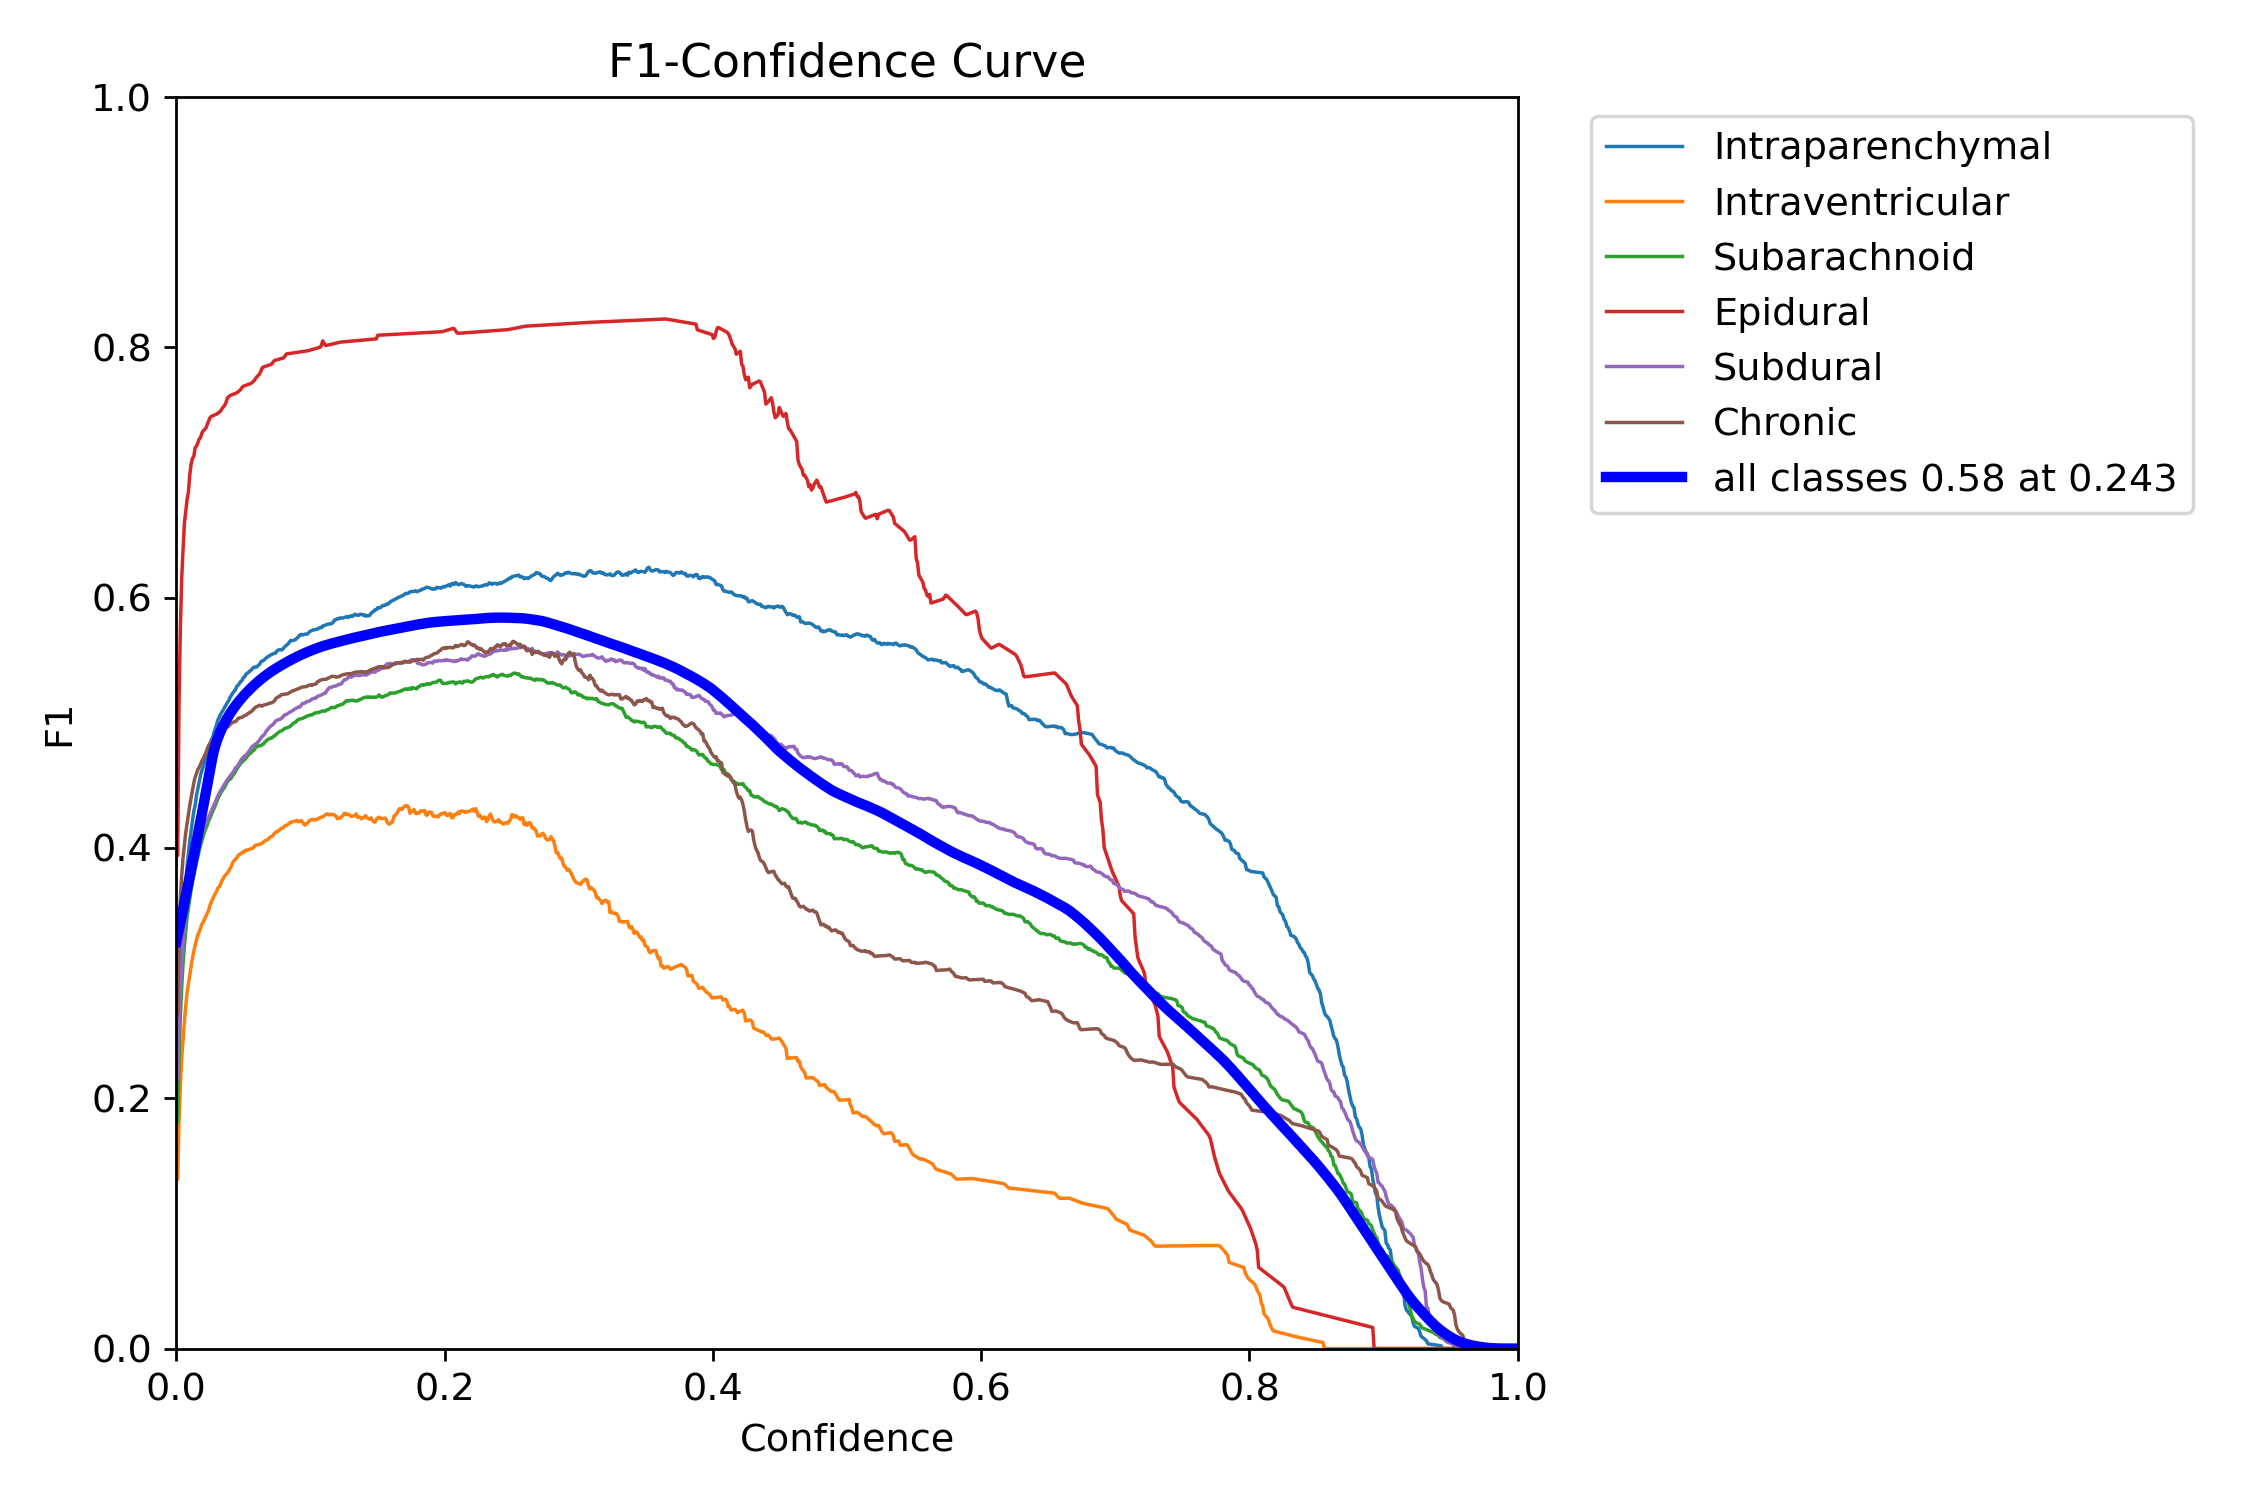
\includegraphics[width=1.0\linewidth]{ISeCure Draft/Images/F1_curve.png}
    \captionsetup{font=small}
    \caption{F1 curve}
    \label{fig:f1}
\end{figure}}

{\begin{figure}[h]
    \centering
    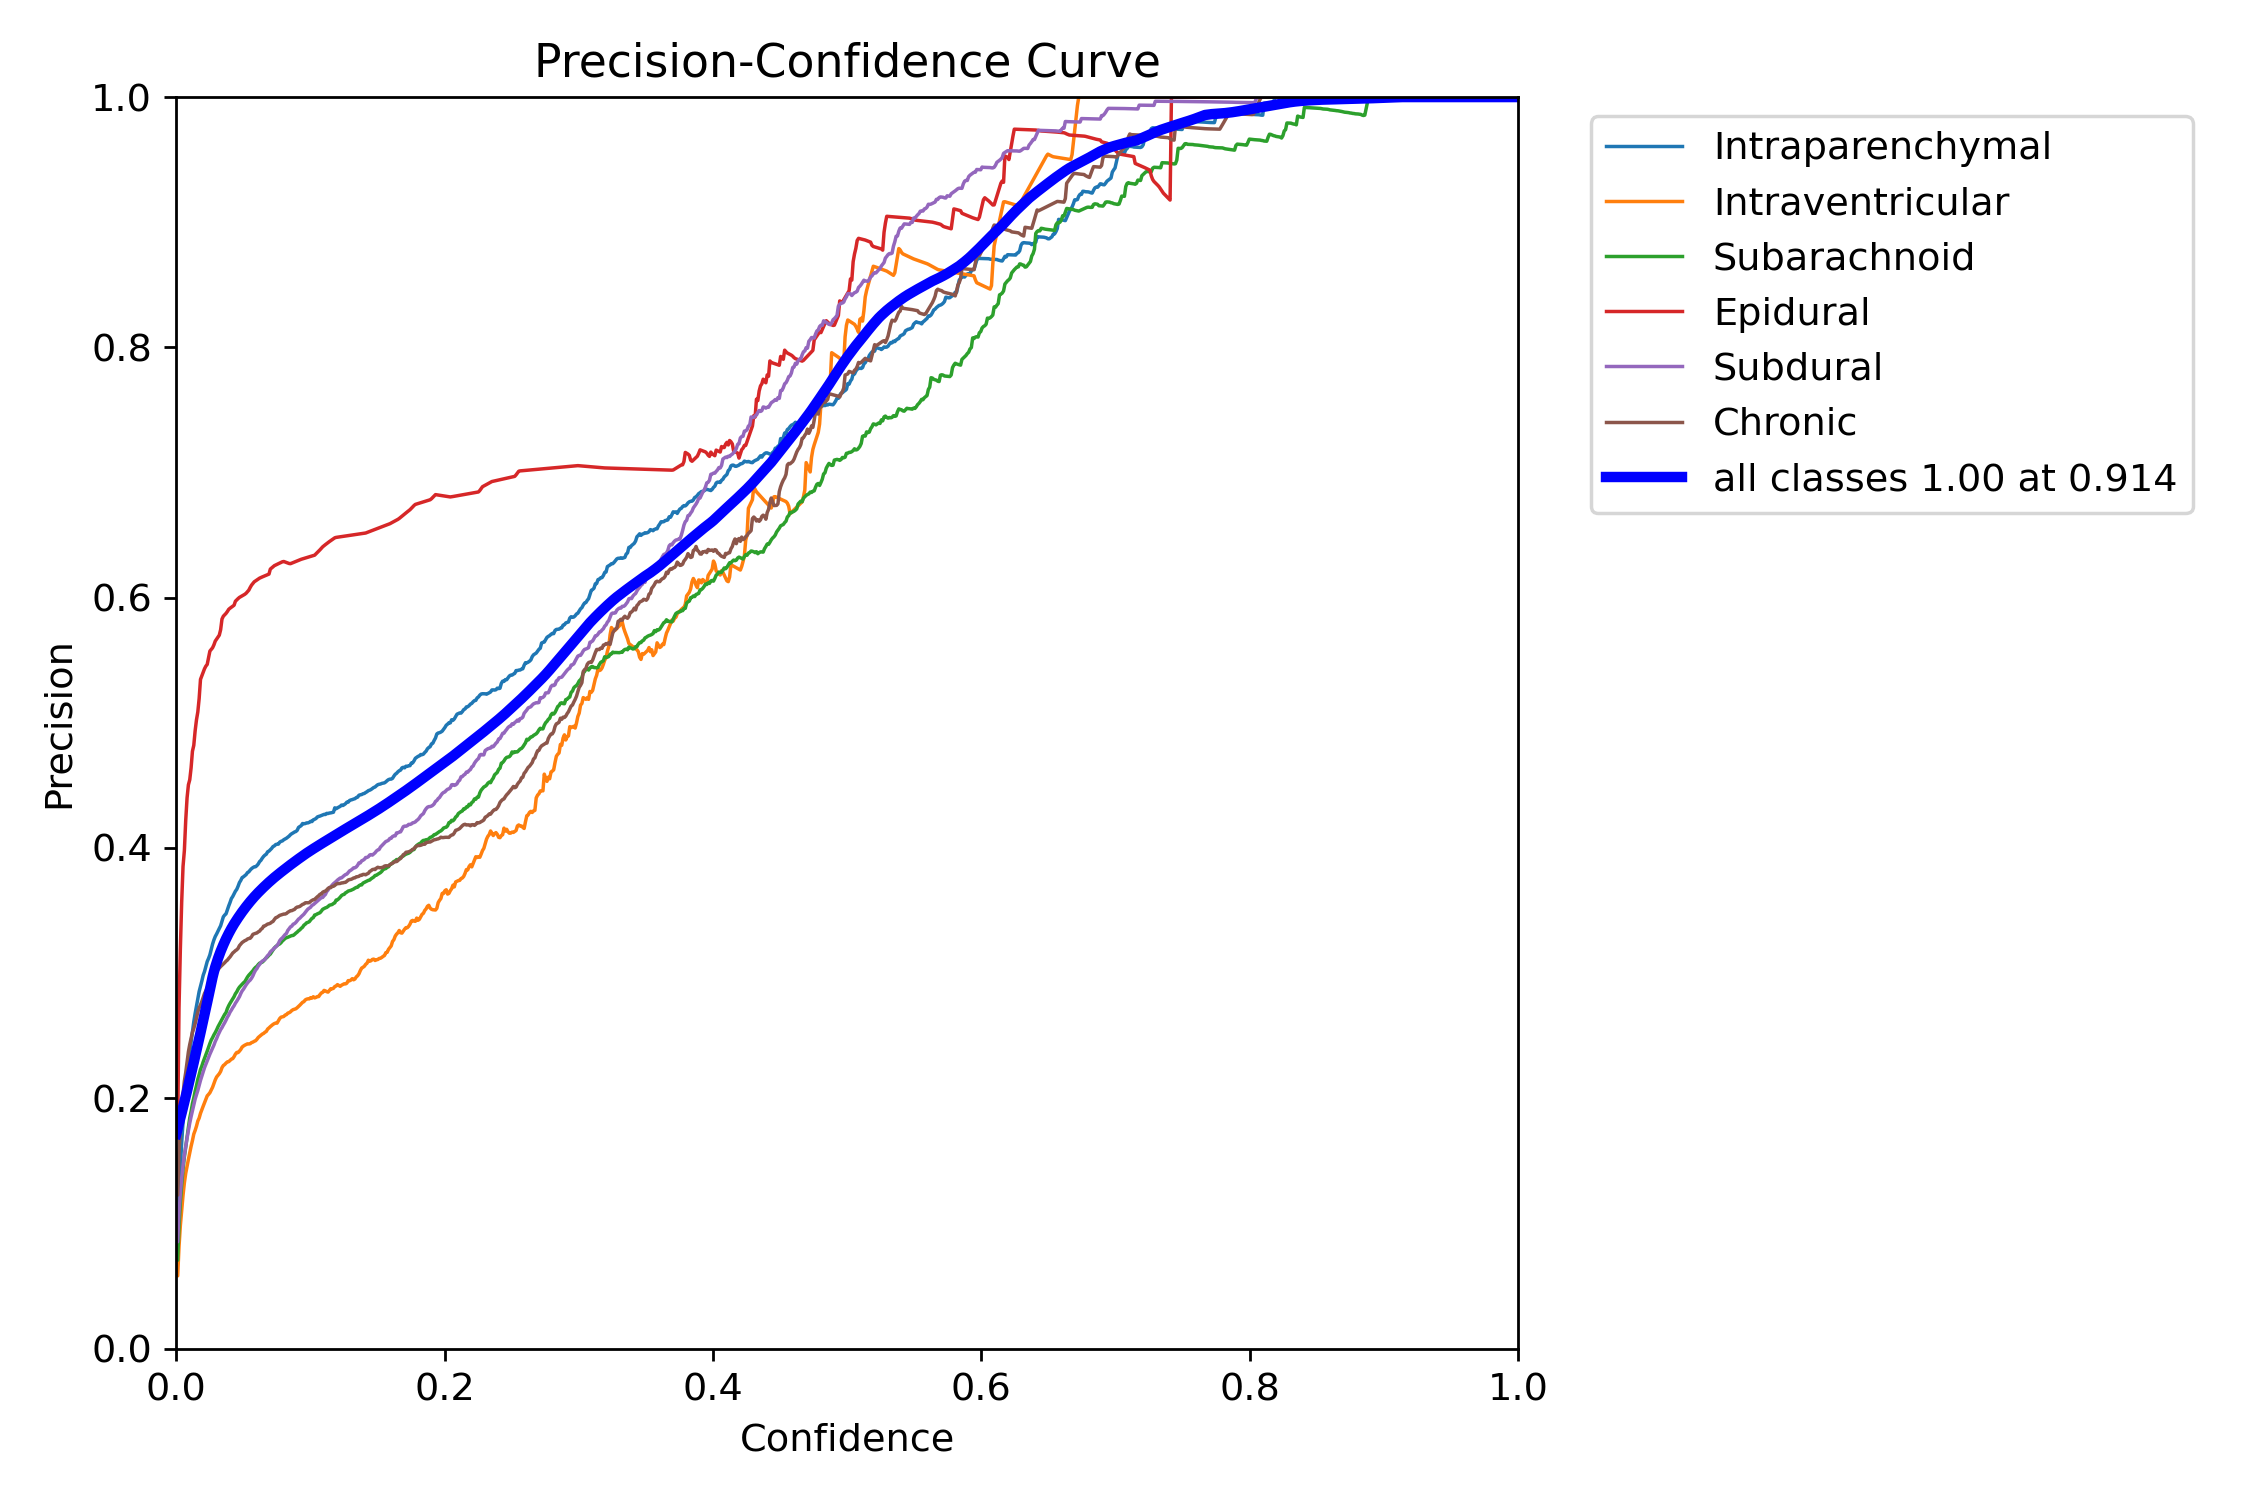
\includegraphics[width=1.0\linewidth]{ISeCure Draft/Images/P_curve.png}
    \captionsetup{font=small}
    \caption{P curve}
    \label{fig:p}
\end{figure}}

{\begin{figure}[h]
    \centering
    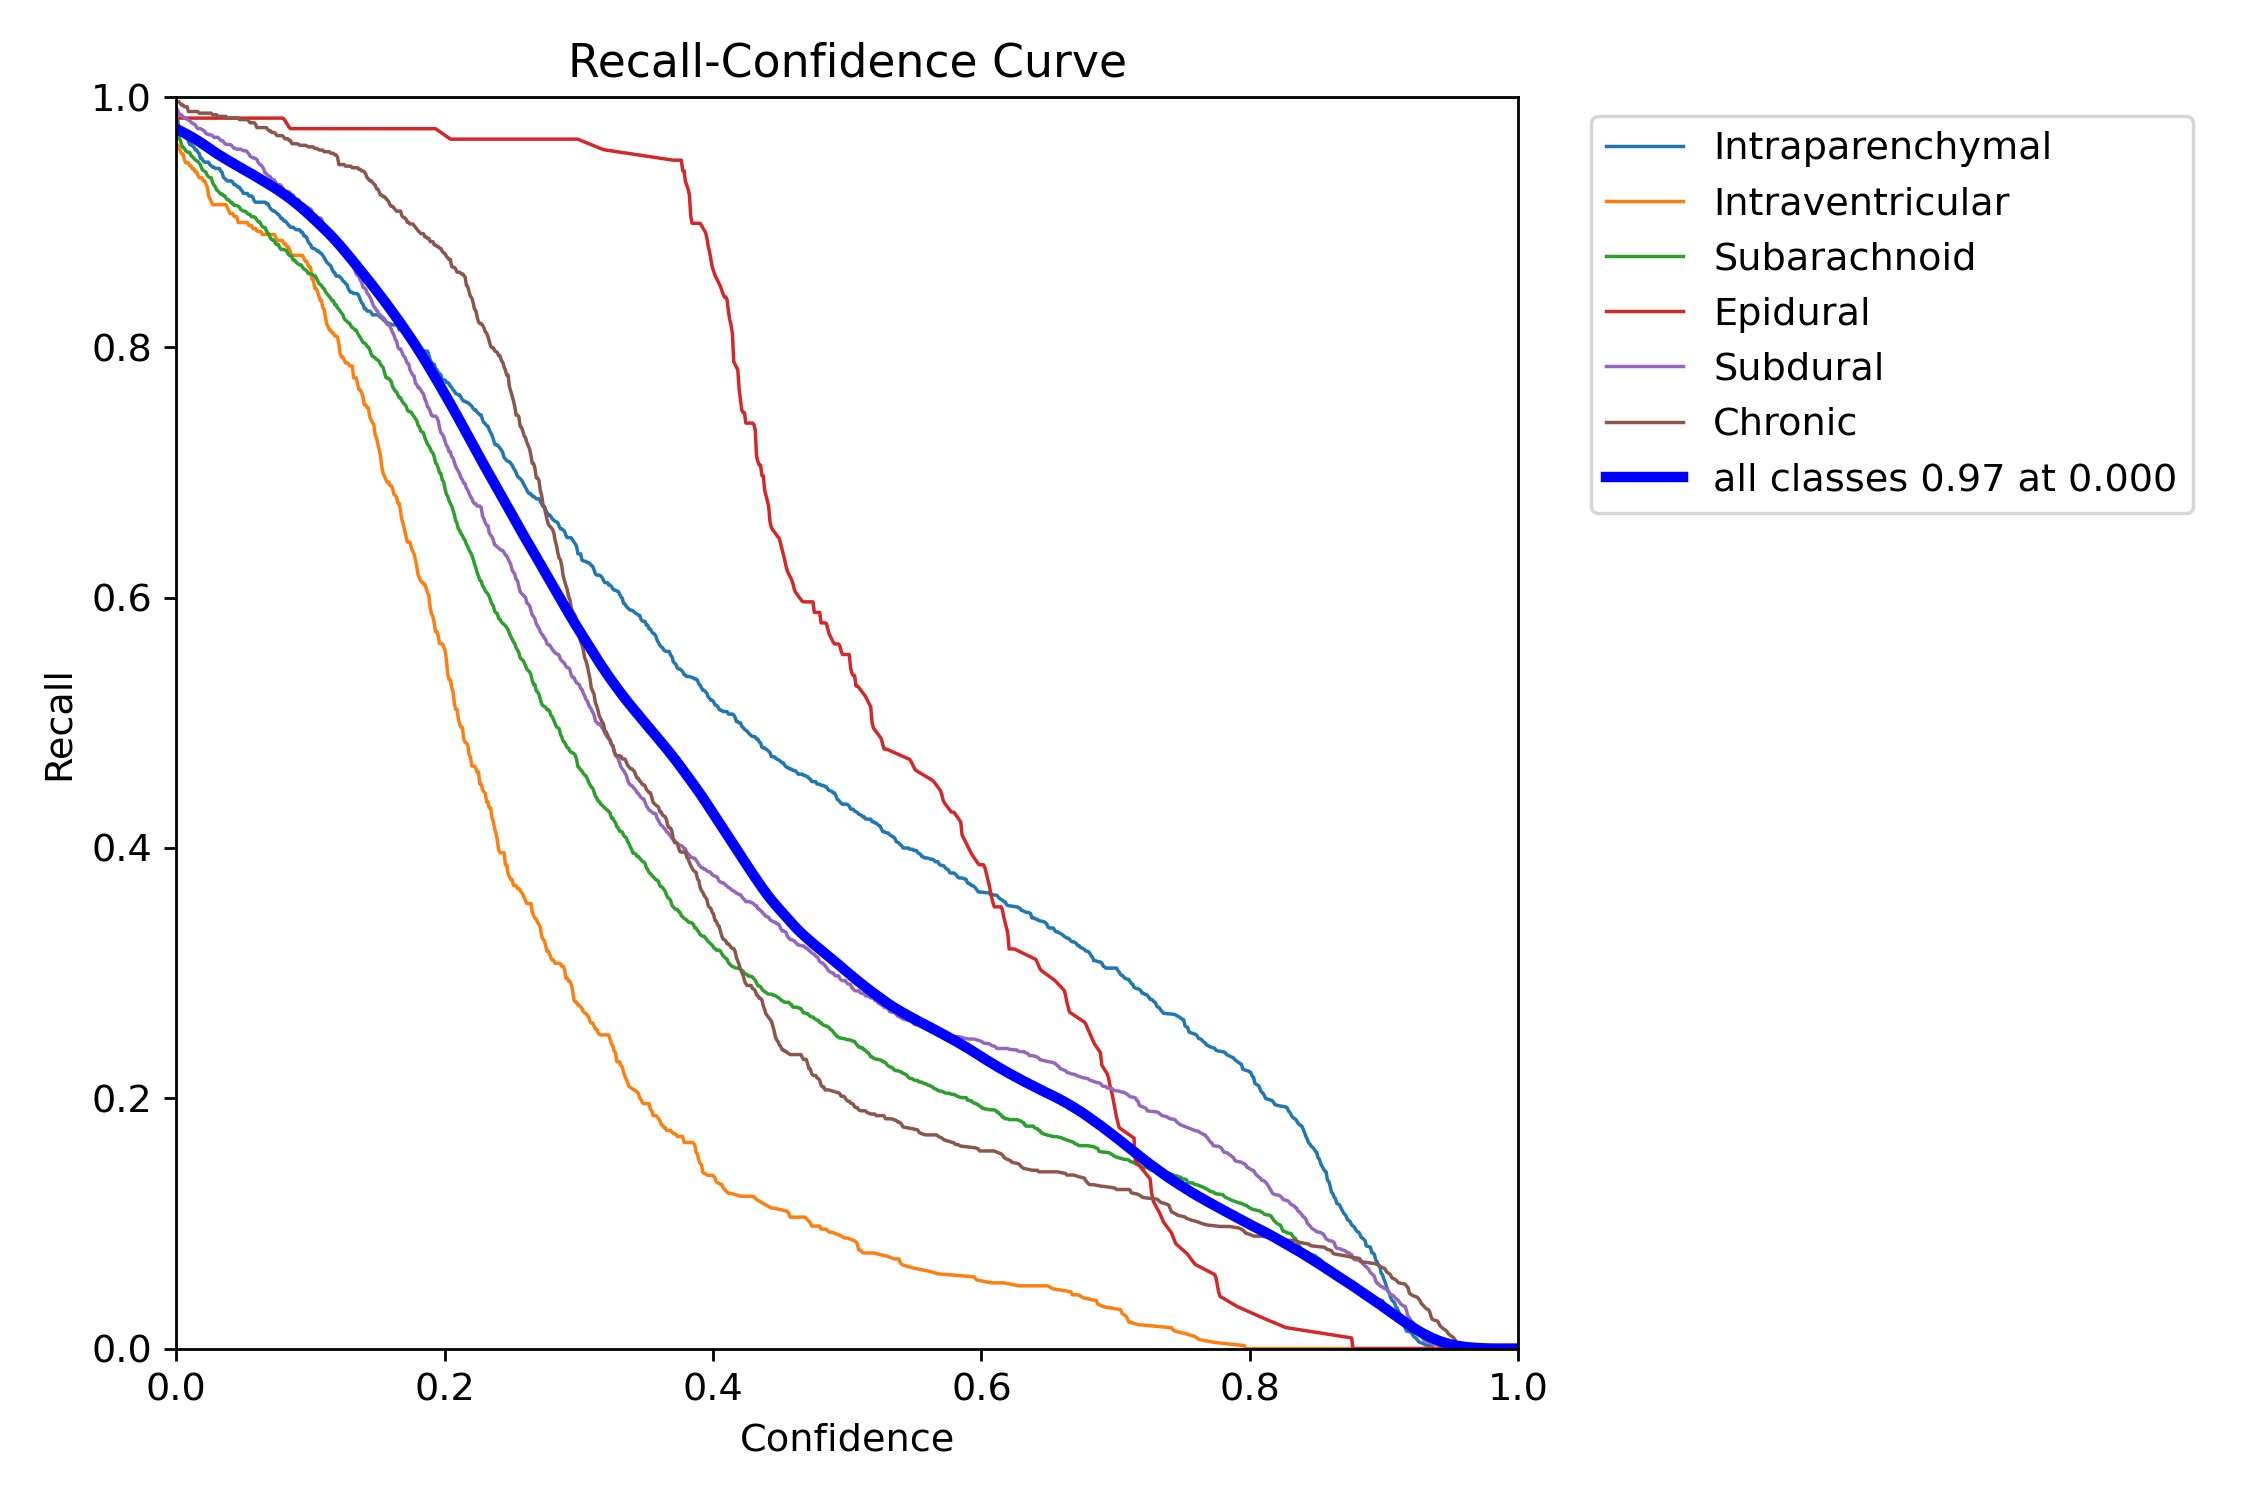
\includegraphics[width=1.0\linewidth]{ISeCure Draft/Images/R_curve.png}
    \captionsetup{font=small}
    \caption{R curve}
    \label{fig:r}
\end{figure}}

{\begin{figure}[h]
    \centering
    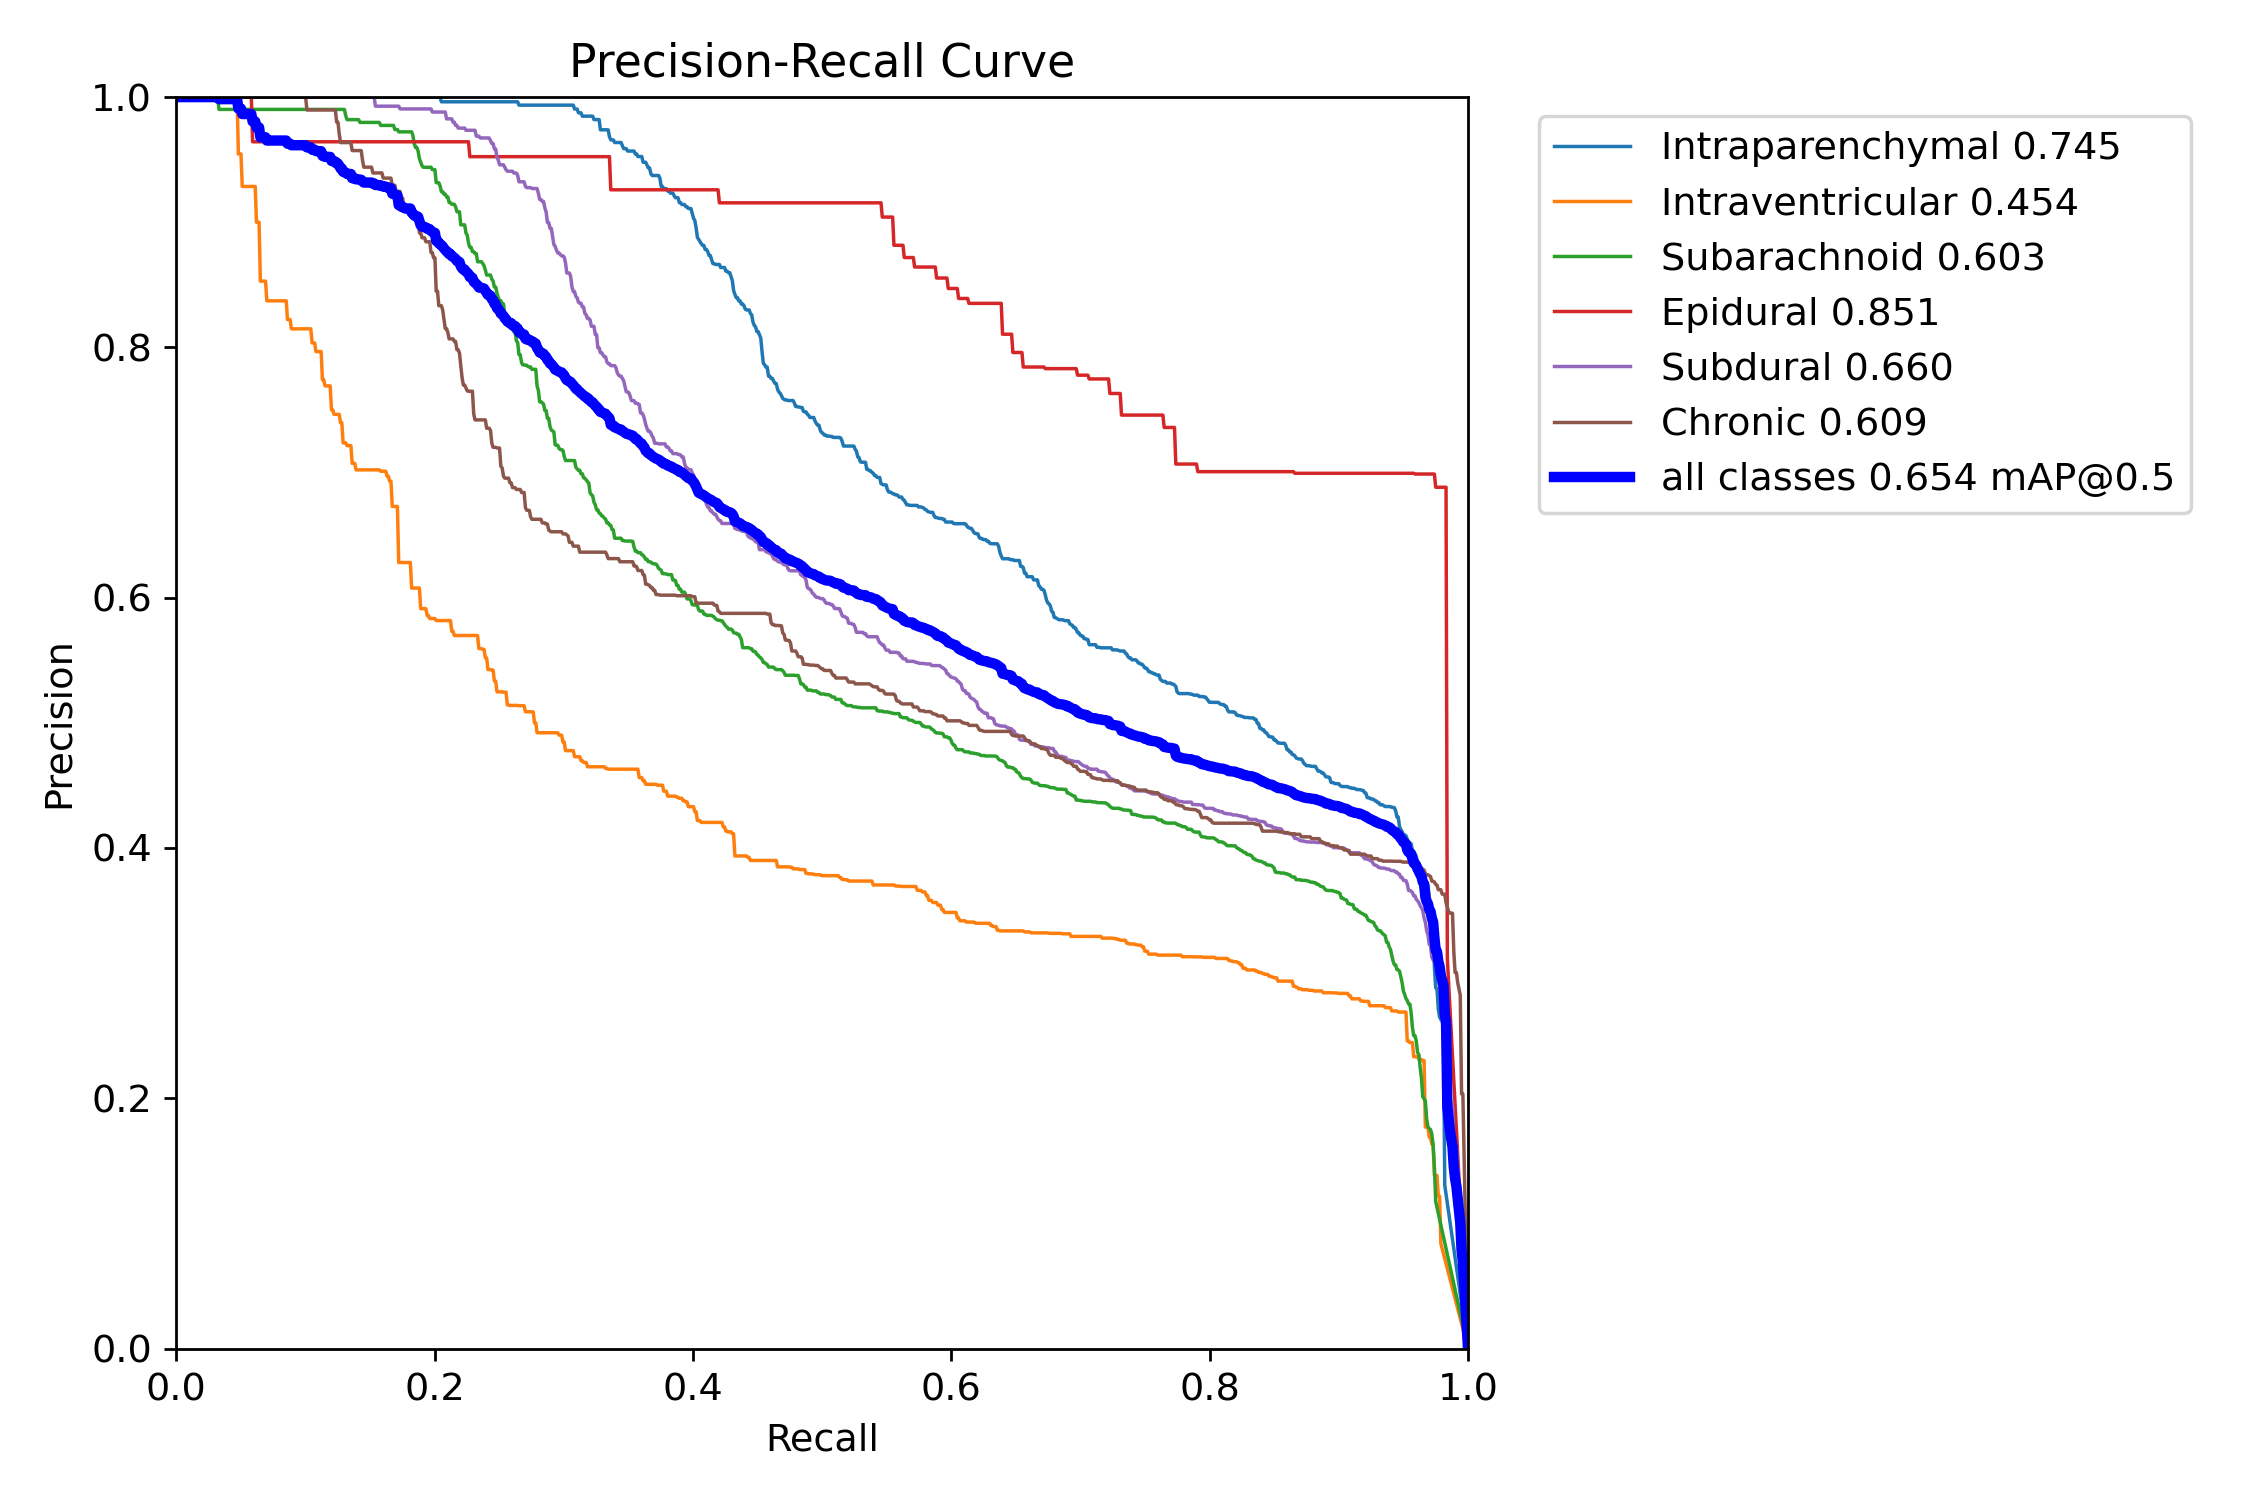
\includegraphics[width=1.0\linewidth]{ISeCure Draft/Images/PR_curve.png}
    \captionsetup{font=small}
    \caption{PR curve}
    \label{fig:pr}
\end{figure}}

{\begin{figure}[h]
    \centering
    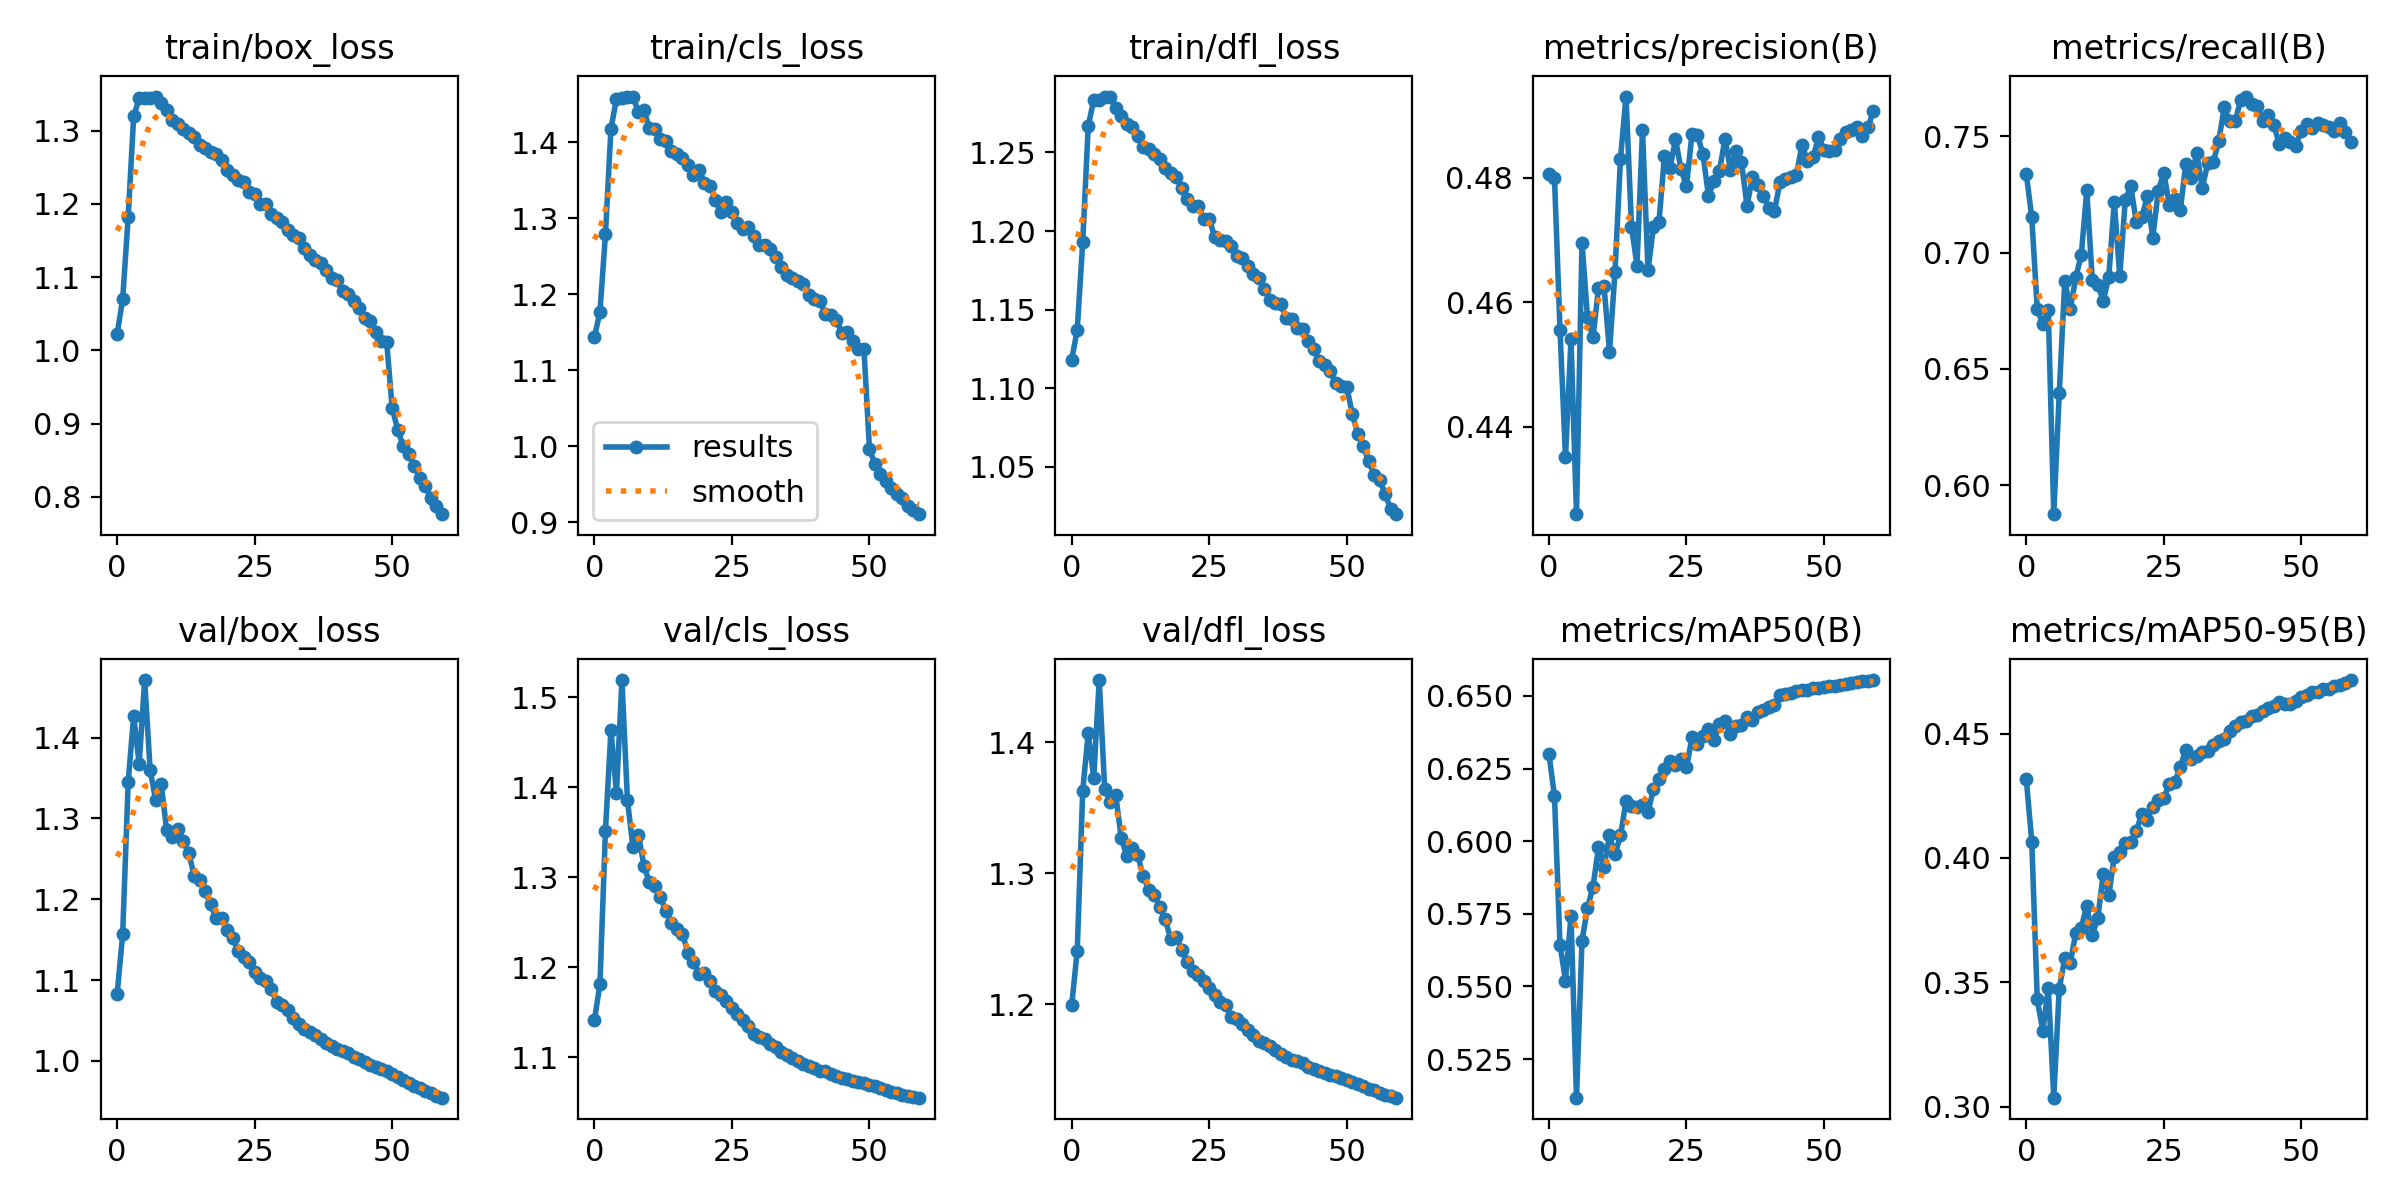
\includegraphics[width=1.0\linewidth]{ISeCure Draft/Images/results.png}
    \captionsetup{font=small}
    \caption{results}
    \label{fig:res}
\end{figure}}

\newpage

\section{Future Work} \label{sec: Future Work}
Future efforts will involve further preprocessing of the image, fine-tuning the model architecture, optimizing parameters for heightened performance, and experimenting with novel methodologies to enhance accuracy. Further iterations with extended training epochs will also be helpful. Addressing class imbalances among various hemorrhage types will be a focal point, ensuring a more equitable and comprehensive dataset. With this, the expectation is to get even lower error rates.



\section{Conclusion}\label{sec:conclusion}
Overall, this project demonstrates the potential of YOLOv8 for detecting and localizing intracranial hemorrhage types in clinical practice. With further development and refinement, this approach could lead to improved diagnostic accuracy and timely patient management. This could be implemented for other areas in healthcare development as well. 

\section*{Acknowledgment}

We express our appreciation to Dr. Ranga Rodrigo and Mr. Tharindu Wickremasinghe for their invaluable guidance and insights.

\begin{thebibliography}{9}  % 9 is the widest number of references you expect

\bibitem{ertugrul2022detecting}
Ömer Faruk Ertuğrul, Muhammed Fatih Akıl,
\emph{Detecting hemorrhage types and bounding box of hemorrhage by deep learning},
\emph{Biomedical Signal Processing and Control}, 
Volume 71, Part A, 2022, 103085,
ISSN 1746-8094, \url{https://doi.org/10.1016/j.bspc.2021.103085}\\
\\

\bibitem{physionet2020bhx}
PhysioNet. (2020). \emph{BHX: Brain Hemorrhage Extended (BHX): Bounding box extrapolation from thick to thin slice CT images.} Retrieved from \url{https://physionet.org/content/bhx-brain-bounding-box/1.1/}\\
\\

\bibitem{heit2017imaging}
Heit, J. J., Iv, M., \& Wintermark, M. (2017). \emph{Imaging of Intracranial Hemorrhage.} \emph{J Stroke}, \textbf{19}(1), 11–27. doi: 10.5853/jos.2016.00563 PMCID: PMC5307932 PMID: 28030895\\
\\

\bibitem{openmmlab2023yolov8}
OpenMMLab. (2023, January 17). \emph{Dive into YOLOv8: How does this state-of-the-art model work?} \emph{Medium}. Retrieved from \url{https://openmmlab.medium.com/dive-into-yolov8-how-does-this-state-of-the-art-model-work-10f18f74bab1#:~:text=In%20summary%2C%20YOLOv8%20is%20a,object%20detection%2C%20and%20instance%20segmentation}


% Add more references if needed

\end{thebibliography}




\end{document}
